\documentclass[a4paper, 11pt]{report}
\usepackage[spanish, activeacute]{babel}
\usepackage{makeidx}
\usepackage{amsmath,amsfonts}
\usepackage{graphicx}
\usepackage{url}
\usepackage{times}
\usepackage{bm}
\usepackage{multicol}
\usepackage{colortbl}

\setlength{\parskip}{7pt plus 2pt minus 1pt}
\addtolength{\topmargin}{-2cm}
\addtolength{\textheight}{4cm}
\makeindex

\begin{document}
\DeclareGraphicsExtensions{.jpg,.pdf,.mps,.png}

\title {
\begin{figure}[h]
\begin{center}

\includegraphics[keepaspectratio, width=3cm]{escudo}
\end{center}
\end{figure}
Universidad de Buenos Aires\\
Facultad de Ciencias Exactas y Naturales\\
Departamento de Computaci\'on\\
\vspace{10mm}
\Huge\textbf{Computaci\'on de alto rendimiento en el estudio de reacciones qu\'imicas en soluciones a trav\'es de m\'etodos cl\'asicos y cu\'anticos.}
\vspace{10mm}
}

\author{por \\
        Pablo Listingart\\
        \\
        Director de Tesis\\
        Lic. Esteban Mocskos\\
        Co-Director de Tesis\\
        Dr. Mariano Camilo Gonzalez Lebrero\\
        \\
        Tesis para optar al grado de \\
        Licenciado en Ciencias de la Computaci\'on\\
        \\
        }
\date{Mayo de 2006}

\maketitle

\tableofcontents

\pagebreak

\begin{center}


{\huge{\textbf{Agradecimientos}}}
\\
\vspace{1cm}

\emph{ A mis padres, Marta y Horacio.}

\emph{A Eli.}

\emph{A Gabi.}

\emph{A mi familia.}

\emph{A Esteban.}

\emph{A Nano y Dar\'io}

\emph{A mis amigos.}

\emph{A la gente del LSC.}

\emph{A los jurados.}

\emph{A todos los que de alguna forma u otra contribuyeron para que yo llegue a este momento.}

\emph{"Imagination is more important than knowledge"}

\emph{Albert Einstein} \vspace{.5cm}

\end{center}
\pagebreak


\maketitle

\chapter*{Resumen \label{Resumen}}
En este trabajo se presenta un software de c\'omputo de alto rendimiento aplicado a la simulaci\'on de reactividad qu\'imica en soluci\'on. 
El m\'etodo utilizado para realizar la simulaci\'on se encuadra dentro de un esquema h\'ibrido cu\'antico-cl\'asico (QM-MM) en el cual el solvente es tratado cl\'asicamente (como masas y cargas puntuales) mientras que el soluto es tratado con rigurosidad cu\'antica (DFT, en nuestro caso), de esta manera se logra optimizar el costo computacional ya que se calcula la estructura electr\'onica s\'olo de la porci\'on del sistema en la que es realmente relevante.
El trabajo consisti\'o en la construcci\'on de un software paralelo de simulaci\'on num\'erica a partir de una versi\'on serial preexistente y su implementaci\'on en una computadora SMP y en un cluster Beowulf para el estudio y predicci\'on de reacciones qu\'imicas en soluci\'on. 
La combinaci\'on del hardware y software mencionado, y el an\'alisis de distintas estrategias de paralelizaci\'on (incluyendo diversas modalidades de pasaje de mensajes) permitieron la resoluci\'on de problemas m\'as realistas y previamente inabordables, obteniendo un algoritmo escalable.

\noindent \textbf{Key Words:} \emph{Beowulf}, \emph{C\'alculo paralelo}, \emph{Cluster}, \emph{DFT}, \emph{M\'etodos h\'ibridos}, \emph{n-body}, \emph{Perfomance}

\pagebreak
\chapter{\strut Introducci\'on \label{Introduccion}}

La simulaci\'on en qu\'imica es una herramienta cada vez m\'as utilizada.
Cuando nos referimos a \emph{simulaci\'on} hablamos del uso de tecnolog\'ia digital para resolver ecuaciones matem\'aticas que definen una teor\'ia particular o un modelo \cite{Cramer}.
El desarrollo de t\'ecnicas refinadas, as\'i como el aumento geom\'etrico del poder de c\'omputo son dos de las razones m\'as importantes de su creciente uso.
Ya sea como complemento o como reemplazo de experimentos, la simulaci\'on aporta, entre otras cosas, una visi\'on microsc\'opica inalcanzable por otra v\'ia.

Por otra parte, la simulaci\'on num\'erica ha crecido de forma considerable en los \'ultimos a\~nos debido a que, desde la perspectiva econ\'omica, el desarrollo te\'orico ha demostrado ser una forma viable de reducir los costos o enfocar m\'as eficientemente la experimentaci\'on.

Las metodolog\'ias utilizadas en simulaci\'on en qu\'imica var\'ian seg\'un el problema a tratar.
En general, se dividen en dos grandes ramas, la llamada rama \emph{cl\'asica} y la llamada \emph{cu\'antica}.
La mec\'anica que rige el comportamiento de part\'iculas peque\~nas (como los electrones) es la llamada mec\'anica cu\'antica, que fue desarrollada a principios del siglo pasado por f\'isicos ilustres como Einstein, Planck, Bhor y otros.

Lamentablemente, no existe una forma exacta de resolver las ecuaciones asociadas a esta mec\'anica, y las soluciones aproximadas accesibles son muy demandantes desde el punto de vista computacional.
Esta elevada demanda hace prohibitivo el uso de esta t\'ecnica a sistemas con un n\'umero elevado de \'atomos.

Por otro lado la mec\'anica cl\'asica, menos demandante, es incapaz de representar electrones, por lo que solo puede utilizarse si la distribuci\'on de los mismos no cambia.
No es posible, entonces, tratar reacciones qu\'imicas (donde la distribuci\'on electr\'onica cambia considerablemente).

Si se quieren tratar reacciones en soluci\'on, se encuentra el problema de que el n\'umero de \'atomos es demasiado grande como para tratarlo con rigurosidad cu\'antica, sin embargo, al haber reacci\'on qu\'imica, no se puede utilizar una metodolog\'ia totalmente cl\'asica.
Por ello se han desarrollado las metodolog\'ias h\'ibridas\cite{Diaz2001,Nemukhin2002,Kesavan2003}, donde a una peque\~na porci\'on del sistema (la parte reactiva), se la trata con la metodolog\'ia cu\'antica, mientras que al resto se lo trata como un campo de fuerzas cl\'asico.

\section{Teor\'ia de los funcionales de la densidad (DFT)}

\subsection{Introducci\'on a la Teor\'ia del Funcional de la Densidad}

En esta tesis se utiliza la teor\'ia del funcional de la densidad (DFT) para el c\'alculo de la estructura electr\'onica en el esquema h\'ibrido cu\'antico-cl\'asico, por este motivo surge la necesidad de realizar una peque\~na rese\~na la misma \cite{Cramer}.

La teor\'ia de los funcionales de la densidad permite obtener la estructura electr\'onica (o cualquier otra propiedad deseada) de un sistema de electrones y n\'ucleos. La idea original, postulada por Thomas y Fermi en la d\'ecada del 20, es contempor\'anea al nacimiento del m\'etodo Hartree-Fock \cite{MCGLPHD,Cramer}, el cual es equivalente en qu\'imica computacional a la aproximaci\'on de orbitales moleculares de enorme utilidad conceptual para los qu\'imicos. Sin embargo debido a su inexactitud a la hora de tratar \'atomos y mol\'eculas, el m\'etodo DFT permaneci\'o relegado hasta mucho despu\'es. Reci\'en en la d\'ecada del 60 Hohenberg y Kohn propusieron dos teoremas \cite{Hohenberg64} que posibilitaron un tratamiento riguroso de la estructura electr\'onica como funcional de la densidad.

Hasta ese momento, la teor\'ia examinada vinculaba la energ\'ia y la densidad electr\'onica, sin embargo no preve\'ia la manera de calcular una u otra. En el a\~no 1965 Kohn y Sham \cite{Kohn65} introdujeron una aproximaci\'on para la forma funcional de la energ\'ia cin\'etica a trav\'es de la cual se hizo posible evaluar la densidad y obtener la
energ\'ia total. Este m\'etodo, denominado de Kohn-Sham, es el que permiti\'o utilizar a DFT como un instrumento de c\'alculo de estructura electr\'onica eficiente. La enorme importancia que adquiri\'o la teor\'ia del funcional de la densidad en qu\'imica se vio reflejada en el otorgamiento del premio Nobel al profesor Kohn en 1998.

\subsection{Descripci\'on de la DFT}

Los m\'etodos tradicionales en la teor\'ia de estructura electr\'onica, en particular Hartree-Fock y sus descendientes, est\'an basadas en una complicada funci\'on de onda para varios electrones \cite{Becke88,Parr89,Koch2002}. 
El objetivo principal de la DFT es reemplazar esta funci\'on de onda por la densidad electr\'onica como base. Mientras que la funci\'on de onda depende de $3N$ variables (tres variables espaciales por cada uno de los N electrones), la densidad es solo funci\'on de tres variables que es mucho m\'as simple para trabajar tanto conceptual como pr\'acticamente.

A pesar de que la DFT tiene sus ra\'ices en el modelo de Thomas-Fermi, como hemos mencionado con anterioridad, no se utiliz\'o realmente hasta que Hohenberg-Kohn propusieron dos teoremas. El primero de ellos demuestra la existencia de un mapeo uno a uno entre la densidad del estado fundamental del electr\'on y la funci\'on de onda del estado fundamental de un sistema con m\'ultiples part\'iculas. En f\'isica, el estado fundamental de un sistema es su estado cu\'antico de menor energ\'ia. El segundo teorema prueba que la densidad del estado fundamental minimiza la energ\'ia electr\'onica total del sistema. Los teoremas originales se mantienen solo para el estado fundamental en ausencia de un campo magn\'etico, aunque los mismos han sido generalizados. El primero de los teoremas es solo uno existencial, aseverando que el mapeo existe, pero no provee ninguno en particular.

Como se menciona anteriormente, la implementaci\'on m\'as com\'un de la DFT es mediante el m\'etodo de Kohn-Sham. Mediante el mismo, el problema $n-body$ de electrones que interact\'uan en un potencial est\'atico externo se ve reducido a un problema de electrones que no interact\'uan y se mueven en un potencial efectivo. Este \'ultimo incluye un potencial externo y los efectos de las interacciones de Coulomb entre los electrones.

DFT se ha convertido en un m\'etodo muy popular desde la d\'ecada del 70 para c\'alculos de estado s\'olido debido a su relaci\'on de costo-calidad sobre otros m\'etodos de resolver el problema $n-body$ en mec\'anica cu\'antica. Sin embargo no fue considerado suficientemente preciso en qu\'imica cu\'antica hasta la d\'ecada del 90 cuando se refinaron las aproximaciones de los mapeos para mejorar el modelado de las interacciones.

DFT es actualmente el m\'etodo m\'as ampliamente utilizado para estructuras electr\'onicas \cite{Estrin,Perdew86,Becke93}. A pesar de las mejoras que ha ido sufriendo todav\'ia existen dificultades para describir adecuadamente algunas interacciones intermoleculares.


\subsection{El modelo Thomas-Fermi}

Como hemos venido mencionando, el predecesor del DFT fu\'e el modelo Thomas-Fermi, que se desarroll\'o en la d\'ecada del 20. Thomas y Fermi calcularon la energ\'ia de un \'atomo representando su energ\'ia cin\'etica como una funci\'on de la densidad electr\'onica, combinando esto con la expresi\'on cl\'asica para las interacciones n\'ucleo-electr\'on y electr\'on-electr\'on.

Aunque este modelo fue un primer paso importante, la ecuaci\'on de Thomas-Fermi ten\'ia una precisi\'on limitada, porque no intentaba representar energ\'ia de canje de un \'atomo predicha por la teor\'ia de Hartree-Fock. Dirac agreg\'o al modelo un funcional de esta energ\'ia reci\'en en 1928.

Sin embargo, la teor\'ia de Thomas-Fermi-Dirac se mantuvo imprecisa para la mayor\'ia de sus aplicaciones. Su mayor causa de error se debi\'o a la representaci\'on de la energ\'ia cin\'etica, seguido por los errores en el intercambio de energ\'ia, y finalmente debido a no tomar en cuenta las correlaciones electr\'onicas.

\subsection{Aplicaciones de DFT}

La teor\'ia de Kohn-Sham se puede aplicar de dos formas distintas, las cuales dependen de lo que se quiera investigar. En el estado s\'olido, se usan bases de onda plana con condiciones de contorno peri\'odicas. Adem\'as, se pone un gran \'enfasis en mantener la consistencia con el modelo idealizado de gas electr\'onico uniforme, que exhibe un comportamiento similar al del s\'olido infinito.

En los estados l\'iquido y gaseoso, el gas de electrones es un mal modelo para el comportamiento de \'atomos y mol\'eculas discretas. Para tratar estos casos se ha desarrollado una enorme variedad de funcionales para aplicaciones qu\'imicas. Algunos de estos funcionales son totalmente inconsistentes con la aproximaci\'on del gas electr\'onico uniforme. A pesar de que los resultados obtenidos con estos funcionales suelen ser suficientemente precisos para la mayor\'ia de las aplicaciones, no existe forma de mejorarlos. Por lo tanto no es posible estimar el error de los c\'alculos sin realizar comparaciones con otros m\'etodos o experimentos, lo cual significa que igualmente deben utilizarse otras t\'ecnicas para comparar con el consiguiente costo que esto significa.



\section{\strut El problema $n-body$}

El problema $n-body$ es aquel de encontrar, dada la posici\'on inicial, masas y velocidades de $n$ cuerpos, sus movimientos siguientes determinados por las leyes de la mec\'anica cl\'asica \cite{NBodyAlgorithms,NBody,Cramer}.

Este problema puede referirse tanto a encontrar tanto los movimientos de cuerpos celestes por medio de la gravedad como los de \'atomos y mol\'eculas debido al potencial el\'ectrico. Usualmente uno tiene un estado inicial, y el problema consiste en ir determinando los estados subsiguientes, para observar como interact\'uan estos cuerpos en el tiempo.

Puede observarse parte de la dificultad del problema $n-body$ analizando inicialmente los casos m\'as sencillos del mismo.
El problema, teniendo dos cuerpos, consiste en estudiar c\'omo interact\'uan los mismos a trav\'es del tiempo.

Si se considera que el centro com\'un de masa de los dos cuerpos esta en reposo, cada cuerpo viaja en una secci\'on c\'onica cuyo foco est\'a en el centro de masa del sistema.

Si ambos cuerpos est\'an ligados, ambos describir\'an elipses en sus trayectorias. La energ\'ia potencial relativa al estar alejados (cuyo valor siempre es negativo) tiene un valor absoluto menor que el total de energ\'ia cin\'etica del sistema (no esta siendo tenida en cuenta la energ\'ia de rotaci\'on sobre sus ejes de los cuerpos).

Si ambos se est\'an alejando, lo har\'an describiendo par\'abolas o hip\'erbolas. En el caso de la hip\'erbola, la energ\'ia potencial tiene un valor absoluto menor que el total de energ\'ia cin\'etica del sistema, por lo tanto la suma de ambas energ\'ias es positiva. En el caso de la par\'abola, la suma de las energ\'ias es igual a cero. Las velocidades tienden tambi\'en a cero a medida que los cuerpos se alejan. El hecho de que la trayectoria parab\'olica no tenga energ\'ia surge de la presunci\'on de que la energ\'ia potencial gravitacional tiende a cero a medida que los cuerpos se alejan infinitamente.

A continuaci\'on se analiza como es el comportamiento del sistema con tres cuerpos.
El mismo es bastante m\'as complicado que el visto anteriormente.
Su soluci\'on puede ser ca\'otica.
En general este problema no puede ser resuelto de forma anal\'itica (en forma de f\'ormula cerrada con constantes conocidas y funciones elementales).
Sin embargo existen soluciones aproximadas que pueden ser calculadas por m\'etodos num\'ericos o de perturbaci\'on.

Un caso especial del problema de tres cuerpos es el llamado $restringido$ que asume que la masa de uno de los mismos es despreciable. Este problema es un caso especial en el cual dos de los tres cuerpos estan en \'orbitas circulares o el\'ipticas.

El problema restringido fue abordado extensamente por muchos matem\'aticos y f\'isicos famosos, como Lagrange en el siglo 18 y Henri Poincar\'e al final del siglo 19.

El trabajo de Poincar\'e en el problema restringido de tres cuerpos result\'o ser la base de la teor\'ia del caos determin\'istico.

El problema que se presenta en este trabajo es similar al $n-body$.
La simulaci\'on de un sistema de part\'iculas es uno de los mayores problemas computacionales tanto en f\'isica como en qu\'imica debido al tiempo que insume.
Para analizar los movimientos de part\'iculas deben primero calcularse los potenciales del sistema en su totalidad.
El potencial en cada punto del sistema es igual a la suma de los potenciales determinados por las part\'iculas. Como puede observarse el costo de este c\'alculo es alto y es por este motivo que se intenta mejorar los tiempos de c\'alculo mediante la paralelizaci\'on del software serial utilizado originalmente, con el objetivo final de permitir utilizarlo en problemas de magnitud creciente.

A pesar de que la problem\'atica con la que se trabaja es muy similar computacionalmente a la que se ha mencionado en esta secci\'on, no se opt\'o en esta etapa del trabajo por aplicar estas estrategias debido a que el programa serial ya estaba utilizando otra t\'ecnica de resoluci\'on y se opt\'o por no cambiar totalmente la misma debido a la incertidumbre sobre los resultados que esto generar\'ia. 
Sin embargo, existe la necesidad de mencionar que existen otras formas de resoluci\'on para situaciones similares. Pueden observarse distintos aspectos del problema en \cite{Cramer,Callahan92,NBody,NBodyAlgorithms}. En la literatura este problema se lo conoce, tambi\'en, como \emph{many-body problem}.


\section{\strut M\'etodos H\'ibridos QM/MM}

Simular reacciones qu\'imicas en soluci\'on requiere la representaci\'on de un gran sistema. En nuestro caso, como se ver\'a  m\'as adelante, se han realizado pruebas con alrededor de 500 mol\'eculas.
Por razones de costo computacional y eficiencia, generalmente estos sistemas son tratados a nivel de mec\'anica molecular (MM)\cite{Leach96,VanDerSpoel98,VanMaaren2001}.
Sin embargo, el mayor problema que tiene la teor\'ia de MM es que no suele ser apropiada para describir procesos que incluyen generaci\'on o rompimiento de v\'inculos tales como las reacciones qu\'imicas.
Para modelar correctamente este tipo de procesos deben utilizarse m\'etodos de mec\'anica cu\'antica (QM)\cite{Szabo89,Mahoney2001}.

La regi\'on del espacio a lo largo de una reacci\'on en la cual ocurren cambios significativos en la estructura electr\'onica generalmente es muy peque\~na comparado con el sistema en su totalidad.
Por lo tanto, lo que se busca es hacer uso de las herramientas de mec\'anica cu\'antica en una regi\'on limitada para modelar el problema, mientras que el resto es modelado mediante mec\'anica molecular (ver figura \ref{fig:Hibrido}) para reducir su complejidad.
Cuando esto ocurre se tiene un h\'ibrido de las metodolog\'ias QM/MM\cite{Cramer,MCGLPHD}.

\begin{figure}[ht!]
\begin{center}
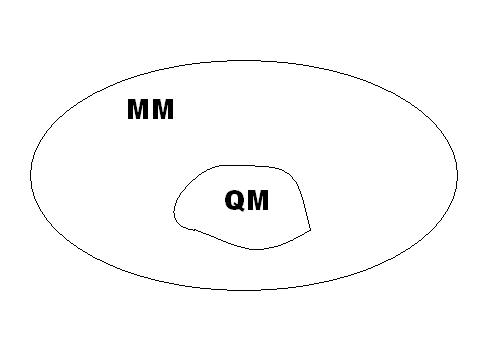
\includegraphics[keepaspectratio, width=10cm]{Hibrido}
\end{center}
\caption[Regiones de un sistema en las cuales se deben aplicar distintas t\'ecnicas.]{\small
{En sistemas grandes, la generaci\'on y rompimiento de v\'inculos puede lograrse mediante la representaci\'on cu\'antica de una peque\~na parte del mismo (Quantum Mechanics, QM), utilizando mec\'anica molecular (Molecular Mechanics, MM) para representar el resto.}}
\label{fig:Hibrido}
\end{figure}

En este tipo de t\'ecnicas la base consiste en combinar c\'alculos de estructura electr\'onica con la mec\'anica molecular cl\'asica a trav\'es de un Hamiltoniano h\'ibrido ($H_{qm-mm}$). En la versi\'on serial del programa modificado en esta t\'esis se utiliz\'o un m\'etodo h\'ibrido $QM/MM$ \cite{Lebrero2005}. Esta combinaci\'on de m\'etodos permite el estudio de sistemas reactivos (que no se pueden tratar con Hamiltonianos cl\'asicos) con un elevado n\'umero de \'atomos (no pueden ser tratados con metodolog\'ias puramente cu\'anticas).

Este m\'etodo propone que es posible escribir la energ\'ia como suma de contribuciones

\begin{displaymath}
E[{R_{i}},{\tau _{a} }] = E_{QM} + E_{QM-MM} + E_{MM}
\end{displaymath}

Donde $E_{QM}$ denota la energ\'ia del subsistema cu\'antico, $E_{MM}$ la del subsistema cl\'asico y $E_{QM-MM}$ es la energ\'ia introducida por la interacci\'on de ambos subsistemas. $R_{i}$ y $\tau _{a}$ son las coordenadas de los n\'ucleos cl\'asicos y cu\'anticos respectivamente.

Un problema importante que presenta esta t\'ecnica es si el l\'imite que separa QM de MM corta alg\'un v\'inculo qu\'imico: si esto no ocurre el modelado es simple. Si, en cambio, se presenta esta situaci\'on la representaci\'on puede convertirse en algo intrincado.

{\huge En tanto que para el segundo parrafo, estaria bueno que haya una figura que muestre los dos ejemplos, sino queda en el aire.}

Mas informaci\'on sobre diversas simulaciones realizadas utilizando m\'etodos QM/MM puede encontrarse en \cite{Kiyohara98,Kusalik94,Svischev96,Yu2004,Stern2001}


% \pagebreak
\chapter{\strut Simulaci\'on num\'erica paralela \label{Simulacion}}

\section{Medici\'on de performance de algoritmos paralelos}

Al desarrollar programas de c\'alculo paralelo, se tiene como objetivo no solo alcanzar la mayor performance posible, sino que la misma se mantenga en proporci\'on a medida que se agregan procesadores al c\'alculo. Para poder tener una noci\'on de la medida de performance de los algoritmos paralelos, se definen las m\'etricas de speedup, eficiencia, overhead y escalabilidad\cite{Pach96,Amdahl,Gustafson88}, que se introducen a continuaci\'on.

\subsection{Speedup}

El Speedup de un programa paralelo, es la relaci\'on entre la versi\'on paralela de un algoritmo, para una cantidad dada de procesadores, y el tiempo de ejecuci\'on de la versi\'on serial del mismo algoritmo. Para poder calcularlo, necesitamos definir primero:

\begin{itemize}
\item $T_1(n)$: Tiempo necesario para la ejecuci\'on de un programa serial, $n$ corresponde a la entrada del programa. \\
\item $T_\mathcal{P}(n,p)$: Tiempo necesario para la ejecuci\'on de la versi\'on paralela del mismo programa con $p$ procesadores.\\
\end{itemize}


Se define entonces como speedup de un programa paralelo corriendo en $p$ procesadores a:

\begin{displaymath}
S(n,p)=\frac{T_1(n)}{T_\mathcal{P}(n,p)}
\end{displaymath}


Esta medida sirve para comparar el rendimiento del algoritmo paralelo con respecto al serial. Cuando $S(n,p) = p$, se dice que se cuenta con un programa de \emph{speedup lineal}.

El speedup lineal es el \'optimo desde el punto de vista de la paralelizaci\'on, puesto que indica una proporci\'on directa y sin desperdicios entre el tiempo de ejecuci\'on y la cantidad de procesadores que intervienen.
Es as\'i que  $0 < S(n,p) \leq p$.
Cuanto mayor sea el speedup de un algoritmo paralelo, mejor ser\'a la performance del mismo en la ejecuci\'on con p procesadores.

\subsection{Eficiencia}

La eficiencia de un programa paralelo, como su nombre lo indica, expresa el aprovechamiento de los recursos de procesador, por parte de dicho programa. Se define como:

\begin{displaymath}
E(n,p)=\frac{S(n,p)}{p}=\frac{T_1(n)}{p*T_\mathcal{P}(n,p)}
\end{displaymath}

de donde se deduce que, para el caso \'optimo de speedup lineal $E(n,p)=1$ .
Para el caso de la eficiencia, las cotas son: $0 < E(n,p) < 1$.
A medida que nuestro valor de eficiencia se acerque a 1, el programa tendr\'a mejor performance.

\subsection{Overhead}

Hay muchos factores que influyen negativamente en los tiempos de ejecuci\'on de un algoritmo paralelo, y son inherentes a la paralelizaci\'on (no existen en un algoritmo serial). Algunos de estos factores son:

\begin{itemize}
\item   Intercambio de mensajes entre los procesos
\item   C\'alculos y decisiones adicionales requeridos en la versi\'on paralela (identificaci\'on de ID, partici\'on en subdominios, etc.)
\item   Tiempos de espera de un proceso (cuando necesita datos de un proceso vecino para poder continuar)
\item   Partes inherentemente seriales del algoritmo (No siempre se puede paralelizar la totalidad del algoritmo)
\end{itemize}

Es por esto, que existe el concepto de \emph{overhead} de un algoritmo paralelo.
Antes de definirlo, necesitamos definir el concepto de $trabajo$ realizado por un algoritmo.
En el caso de un algoritmo serial, el trabajo realizado por el mismo, es simplemente el tiempo que se necesita para su ejecuci\'on:

\begin{displaymath}
W_1(n)=T_1(n)
\end{displaymath}

Cuando se trata de un algoritmo paralelo, el trabajo realizado por el mismo es la suma del trabajo de cada uno de los procesadores:

\begin{displaymath}
W_\mathcal{P}(n,p)=\sum_{i=1}^{p}W_i(n,p)
\end{displaymath}

Donde $W_i(n,p)$ es el trabajo realizado por el programa ejecutado en el procesador $i$.
Puesto que los tiempos de espera en cada procesador forman parte de su trabajo, resulta que  $W_i(n,p)=T_\mathcal{P}(n,p)$, es decir que cada uno de los procesos tarda el tiempo total en terminar (haciendo algo \'util o no).
Con lo cual:

\begin{displaymath}
W_\mathcal{P}(n,p)=\sum_{i=1}^{p}W_i(n,p)=\sum_{i=1}^{p}T_{\mathcal{P}_i}(n,p)=p * W_i(n,p)
\end{displaymath}

Con estas definiciones, decimos entonces que el overhead de un programa paralelo es el trabajo adicional que dicho programa realiza respecto a la soluci\'on serial equivalente:

\begin{displaymath}
T_\mathcal{O}(n,p) = W_\mathcal{P}(n,p) - W_1(n)=p * T_\mathcal{P}(n,p) - T_1(n)
\end{displaymath}

El overhead, que est\'a presente en todos los algoritmos paralelos, es el responsable de no poder lograr un \emph{speedup lineal}.
Al dise\~nar algoritmos paralelos, se trabaja para minimizar el overhead y poder lograr as\'i un aumento del speedup.


\section{L\'imites te\'oricos de la performance de un algoritmo paralelo}

Si bien la paralelizaci\'on de un algoritmo provee un aumento de la performance con respecto al algoritmo serial, este aumento no es necesariamente ilimitado. Inicialmente, Amdahl \cite{Amdahl} evalu\'o que la m\'axima eficiencia que un algoritmo paralelo puede lograr, con respecto a su soluci\'on serial, est\'a sujeta a la proporci\'on paralelizable del algoritmo serial y no depende de la cantidad de procesos que intervengan en el c\'alculo. Esto es conocido como \emph{Ley de Amdahl}.

Posteriormente, Gustafson \cite{Gustafson88} re-evalu\'o la ley de Amdahl, considerando que un problema paralelo puede \emph{agrandarse} para mantener la performance a medida que se aumentan los procesadores.
A continuaci\'on se mencionan ambos estudios.

\subsection{Ley de Amdahl}

Al analizar cualquier algoritmo paralelo, se encontrar\'a que al menos una parte del mismo es inherentemente secuencial. Esto limita el speedup que se puede obtener por medio de la utilizaci\'on de una computadora paralela.
Si la fracci\'on del problema que es inherentemente secuencial es f, entonces el m\'aximo speedup que se puede obtener en una computadora paralela es 1/f. Esto es, el tiempo de ejecuci\'on de la soluci\'on paralela ser\'a:

\begin{displaymath}
T_\mathcal{P}(n,p)=f * T_1(n)+\frac{(1-f)T_1(n)}{p}
\end{displaymath}

Y por lo tanto, el factor de speedup ser\'a:

\begin{displaymath}
S(n,p)=\frac{T_1(n)}{T_\mathcal{P}(n,p)} = \frac{T_1(n)}{f * T_1(n) + \frac{(1-f) T_1(n)}{p}}= \frac{1}{\frac{p*f+(1-f)}{p}}=\frac{p}{1 + (p-1) f}
\end{displaymath}

Luego, a\'un contando con infinitos procesadores, el m\'aximo speedup que se puede obtener est\'a limitado por $1 / f$.

\begin{displaymath}
\lim_{p \to \infty} S(n,p)=\frac{1}{f}
\end{displaymath}

A su vez, la eficiencia de un programa paralelo se acercar\'a a cero a medida que se incorporen nuevos procesadores, puesto que

\begin{displaymath}
\lim_{p \to \infty} E(n,p) = \lim_{p \to \infty} \frac{S(n,p)}{p} = 0
\end{displaymath}

De acuerdo con la Ley de Amdahl y a modo de ejemplo, resulta que si un problema es solo 5\% serial, el m\'aximo speedup que se puede obtener con una soluci\'on paralela es 20, independientemente de la cantidad de procesadores que se utilicen.

\subsection{Ley de Gustafson}

Gustafson, presenta un argumento para mostrar que la ley de Amdahl no es tan significativa como se pensaba con anterioridad, en limitar el speedup potencial de una soluci\'on paralela.
Este argumento se basa en la observaci\'on de que una computadora paralela de mayor tama\~no, permite ejecutar un problema de mayor tama\~no tambi\'en, en un tiempo razonable.

De esta forma, se propone mantener fijo el tiempo de ejecuci\'on, pero incrementar el tama\~no del problema y la cantidad de procesadores de la computadora paralela.
Es as\'i que, manteniendo constante el tiempo de ejecuci\'on, entonces el factor de speedup resultar\'a diferente al que define Amdahl y se denomina \emph{factor de speedup escalado}.

La ley de Gustafson se expresa de la siguiente forma: Sea $s$ la fracci\'on inherentemente serial de un algoritmo paralelo, y sea $p$ la fracci\'on paralelizada.
Si se fija de forma constante en $s + p$ el tiempo de ejecuci\'on en un procesador, y para simplificar la explicaci\'on, se asume que $s + p = 1$. entonces, la ley de Amdahl establece que:

\begin{displaymath}
S(n)=\frac{s+p}{s+p/n}=\frac{1}{s+(1-s)/n}
\end{displaymath}


(Nota: En este caso, la cantidad de procesadores est\'a denotada por n).

Para utilizar el factor de speedup escalado que define Gustafson, se considera constante el tiempo de ejecuci\'on en paralelo en lugar del tiempo de ejecuci\'on serial. Ahora $s + p$ (la parte serial y paralela del programa, respectivamente) ser\'a el tiempo de ejecuci\'on en la computadora paralela y, nuevamente, para simplificar la explicaci\'on, se asume que $s+p=1$.

Entonces, el tiempo que requiere la ejecuci\'on en una \'unica m\'aquina para resolver el mismo problema es $s+n p$, puesto que la parte paralela debe ejecutarse en forma secuencial.
El speedup escalado ser\'a:

\begin{displaymath}
S_{s}(n)=\frac{s+np}{s+p}=s+np=s+n(1-s)=n+(1-n)s
\end{displaymath}


\section{Arquitecturas paralelas}
A continuaci\'on haremos un breve repaso de los paradigmas de programaci\'on paralela existentes al momento de encarar este trabajo. Luego, explicaremos m\'as detalladamente el paradigma de \textit{message-passing}, que es el que utilizamos para la implementaci\'on de la soluci\'on paralela de nuestro problema.

\subsection{Arquitectura MIMD}

Multiple-instruction-multiple-data es la clasificaci\'on en la taxonom\'ia de Flynn para un procesador paralelo(una computadora con m\'as de una unidad de procesamiento central usada para procesamiento paralelo) donde varias unidades funcionales(subsistemas de la CPU) realizan diferentes operaciones sobre datos distintos. Un ejemplo es una red de estaciones de trabajo.

La taxonom\'ia de Flynn define las siguientes categor\'ias
\begin{itemize}
\item Single instruction/single data stream (SISD) - Computadora secuencial.
\item Multiple instruction/single data stream (MISD) - Inusual debido a que no tiene mucho sentido pues generalmente m\'ultiples instrucciones requieren de m\'ultiples datos para ser efectivas. Sin embargo, esta arquitectura se utiliza en algunas m\'aquinas en las que se necesita paralelismo redundante. 
\item Single instruction/multiple data streams (SIMD) - Por ejemplo un \emph{array processor}.
\item Multiple instruction/multiple data streams (MIMD) - m\'ultiples procesadores aut\'onomos ejecutando simult\'aneamente diferentes instrucciones sobre diferentes datos.
\end{itemize}


\subsection{Message passing (Pasaje de mensajes)\label{message passing}}

\textit{Message-passing} consiste en un grupo de procesos que se comunican entre s\'i por medio del intercambio de mensajes para realizar una tarea determinada. En esta implementaci\'on hemos utilizado la biblioteca standard MPI\ (Message Passing Interface) \cite{Pach96, Gropp94} sobre una arquitectura Beowulf \cite{Beowulf}.

Un cluster Beowulf es un conjunto de computadoras personales, no necesariamente homog\'eneas, interconectadas en red que comparten sus recursos de procesamiento y almacenamiento y pueden funcionar cooperativamente y en forma sincronizada para la ejecuci\'on de algoritmos paralelos dise\~nados especialmente.
Estas computadoras, en comparaci\'on con las supercomputadoras de alta performance, tienen un costo mucho m\'as accesible, ampliando las posibilidades de equipamiento de los investigadores e instituciones educativas.
La posibilidad de coexistencia de diferentes modelos de procesadores y hardware, simplifican la escalabilidad de un cluster Beowulf.

En un cluster Beowulf, cada computadora o procesador se denomina $nodo$.
De esta forma, se puede abstraer la arquitectura del mismo, a\'un en los casos de contar tanto con computadoras monoprocesador como multiprocesador en el mismo cluster.
Aqu\'i se asume que en cada procesador f\'isico se corre un solo proceso.

Existen diversas aplicaciones de administraci\'on de procesos y aplicaciones en clusters Beowulf, muchas de ellas gratuitas y de c\'odigo abierto. Las m\'as importantes que se utilizan en el Laboratorio de Sistemas Complejos\cite{LSC} son:

\begin{itemize}
\item   PBS: Administrador de recursos de un cluster. Se utiliza para establecer pol\'iticas sobre la asignaci�n y utilizaci\'on de los recursos (principalmente procesadores) de un cluster. Provee colas de procesos, herramientas para encolar, visualizar y desencolar procesos, herramientas de monitoreo, etc.\cite{PBS}
\item   MAUI Scheduler: Encolador avanzado de procesos. Se encarga de administrar la cola de procesos, para permitir la aplicaci\'on de prioridades, l�mites de ejecuci\'on, permisos, etc. \cite{MAUI}
\end{itemize}


% \pagebreak
\chapter{Metodolog\'ia \label{Metodologia}}

El desarrollo de un programa paralelo tiene como objetivo no s\'olo optimizar una \'unica m\'etrica, como puede ser el tiempo de ejecuci\'on total.
Un buen dise\~no debe, adem\'as, optimizar una funci\'on dependiente del problema a resolver donde se tienen en cuenta el tiempo de ejecuci\'on, los requerimientos de memoria, los costos de implementaci\'on y mantenibilidad de la soluci\'on, entre otros.
Estas optimizaciones en el dise\~no conllevan una tensi\'on entre simplicidad, performance, portabilidad y otros factores.

Partiendo de un programa serial pre existente \cite{lebrero2002} y para poder decidir c\'omo encarar estas optimizaciones, se debi\'o realizar un estudio de la complejidad y del comportamiento del programa serial.
Para ello se realiz\'o un profiling utilizando diversas herramientas provistas por el sistema operativo Linux y por el compilador $g77$ utilizado (son descriptas m\'as adelante).

Como ya fue mencionado, en la versi\'on serial se utiliz\'o un m\'etodo h\'ibrido $QM/MM$ \cite{Lebrero2005}.
Mediante la combinaci\'on de m\'etodos cu\'anticos y cl\'asicos es posible el estudio de sistemas reactivos (que no se pueden tratar con Hamiltonianos cl\'asicos) con un elevado n\'umero de \'atomos (no pueden ser tratados con metodolog\'ias puramente cu\'anticas).

Sepuede observar en el cap\'itulo \ref{Introduccion} que el m\'etodo QM/MM describe la energ\'ia como suma de contribuciones

\begin{displaymath}
E[{R_{i}},{\tau _{a} }] = E_{QM} + E_{QM-MM} + E_{MM}
\end{displaymath}

Esta f\'ormula indica que el total de enrg\'ia del sistema es equivalente a la suma de energ\'ia del subsistema cu\'antico ($E_{QM}$), la del subsistema cl\'asico ($E_{MM}$)  y la energ\'ia introducida por la interacci\'on de ambos subsistemas ($E_{QM-MM}$).

La energ\'ia correspondiente al subsistema cu\'antico puede calcularse con cualquier m\'etodo de estructura electr\'onica. De la misma manera cualquier campo de fuerzas cl\'asico puede aplicarse al subsistema correspondiente.

Como se mencion\'o con anterioridad, el esquema de aproximaci\'on implementado en la versi\'on serial est\'a basado en la teor\'ia del funcional de la densidad (DFT) por su buena relaci\'on costo-calidad, en la cual la variable fundamental es la densidad electr\'onica.
Esta variable, $\rho$, se expande con un conjunto de funciones base.

\begin{displaymath}
\rho = \sum_{i=1}^N \mid X_i^{KS} \mid^{2}
\end{displaymath}

Se puede escribir la energ\'ia total como:

\begin{displaymath}
E[\rho] = -\frac{1}{2}\langle X_i^{KS}\mid \sum_i\sigma_i^{2} \mid X_i^{KS}\rangle + \int v(r) \rho(r) dr + \frac{1}{2}\int \int \frac{\rho(r_{1})\rho(r_{2})}{r_{12}}dr_{1}dr_{2}+E_{xc}[\rho]
\end{displaymath}

La parte m\'as costosa del c\'alculo esta relacionada con los dos \'ultimos t\'erminos de esta expresi\'on, que corresponden a la energ\'ia de repulsi\'on de Coulomb, y el t\'ermino de intercambio y correlaci\'on.

El primer t\'ermino es calculado en forma anal\'itica, pero su costo del orden de $N^3$, donde $N$ est\'a directamente relacionada con el tama\~no del sistema.
Este t\'ermino consiste de $N^3$ integrales anal\'iticas que se pueden calcular en forma independiente, por lo que se puede paralelizar con facilidad.

El segundo t\'ermino se debe evaluar en forma num\'erica, empleando un esquema de integraci\'on en una grilla centrada en los \'atomos y tambi\'en escala como $N^3$.
Este t\'ermino es paralelizable entre los distintos procesos separando el dominio sobre el que se calcula la integral.

En el profiling realizado veremos que el c\'omputo de estos dos t\'erminos representa m\'as del 90\% del costo computacional total, ya que el costo de los dos primeros t\'erminos escala con $N^2$.

\section{Profiling}

Para obtener un profiling de un programa se cuenta con distintas herramientas, a nivel sistema operativo y a nivel compilador. Detallamos a continuaci\'on aquellas que hemos utilizado.

\begin{itemize}
\item  Comando {\it time}

Este es un comando provisto por los sistemas operativos basados en Unix que recolecta datos b\'asicos sobre la performance y la utilizaci\'on de recursos de un programa.

Corriendo un programa con el comando {\it time}, a su terminaci\'on se obtiene una l\'inea con informaci\'on de los tiempos y recursos utilizados.

Por ejemplo:

{\bf demo\% time miprograma}

a la terminaci\'on del programa se obtiene por ejemplo:

{\bf demo\% 451.48 user 0.53 system 7:49.20 elapsed 96\%CPU (0 avgtext + 0 avgdata 0 maxresident) k 0inputs + 0 outputs (1109 major + 3084 minor) pagefaults 0 swaps}


Donde la interpretaci\'on es la siguiente:
\begin{itemize}
\item {\it User}: 451.48 segundos de c\'odigo de usuario
\item {\it System}: 0.53 segundos de c\'odigo de sistema
\item {\it Wallclock}: 7:49.20 minutos para completar el procesamiento completo
\item {\it Recursos}: 96\% de uso de CPU
\item {\it Memoria}: (0avgtext+0avgdata 0maxresident)k
\item {\it I/O}: 0 lecturas, 0 escrituras
\item {\it Paginaci\'on}: (1109major+3084minor)pagefaults, 0 swaps
\end{itemize}

\item  Comando {\it gprof}

El comando {\it gprof} provee un an\'alisis postmortem de tiempos a nivel de subrutinas, incluyendo cu\'antas veces una subrutina fue llamada, por qui\'en fue llamada, y cu\'anto tiempo fue insumido por cada subrutina y las llamadas por \'esta .

Para activar la opci\'on de este tipo de profiling se debe compilar el programa con los flags \texttt{-gp}.

\texttt{demo\% f77 -o miprograma -pg miprograma.f }...etc

Luego, se ejecuta el programa normalmente.
Esta ejecuci\'on va a generar autom\'aticamente un archivo \texttt{gmon.out} con todos los datos de profiling.

Luego se ejecuta:

\texttt{demo\% gprof miprograma}

y se obtiene como resultado un reporte con el an\'alisis completo.

\item Comando {\it tcov}

El comando {\it tcov} produce un profiling de un nivel m\'as interno, ya que recolecta informaci\'on sentencia por sentencia del programa fuente, mostrando como resultado cu\'antas veces se ejecut\'o cada sentencia durante una corrida completa.
Tambi\'en produce informaci\'on sobre la estructura b\'asica de los bloques del programa.

Para activar la opci\'on de este tipo de profiling se debe compilar el programa con los flags {\it -a, -xa }o{\it -xprofile=tcov}.

{\bf demo\% f77 -a -o miprograma miprograma.f ...etc }

Luego, se ejecuta el programa normalmente. Esta ejecuci\'on va a generar autom\'aticamente un archivo {\it .d} por cada archivo {\it .f}. Para ver la informaci\'on de profiling se ejecuta el comando {\it tcov} sobre los archivos fuentes:

{\bf demo\% tcov miprograma.f}

Como output de este comando se obtiene, finalmente, un archivo {\it .tcov} por cada archivo fuente. Estos archivos son una versi\'on anotada del c\'odigo donde adelante de cada sentencia se especifica la cantidad de veces que fue ejecutada.

\end{itemize}


A continuaci\'on observaremos los datos obtenidos de la realizaci\'on del profiling del programa serial.
En la figura \ref{fig:Profiling} se detallan los porcentajes de procesamiento que insume cada subrutina en una corrida.

\begin{figure}[ht!]
\begin{center}
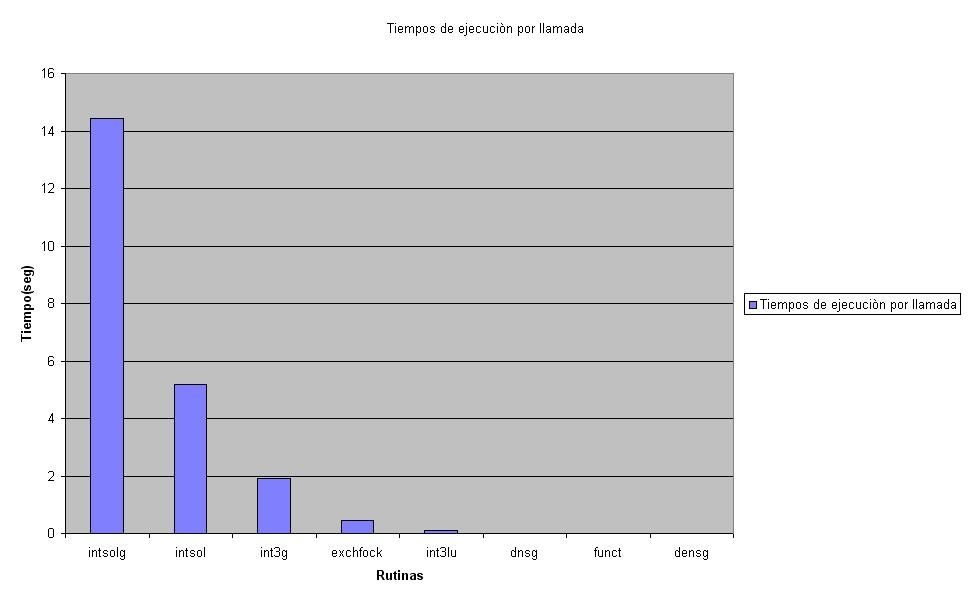
\includegraphics[keepaspectratio, width=14cm]{tiempos}
\end{center}
\caption[Tiempo consumido por las rutinas]{\small{Tiempo consumido por las rutinas.}}
\label{fig:tiempos}
\end{figure}

\begin{figure}[ht!]
\begin{center}
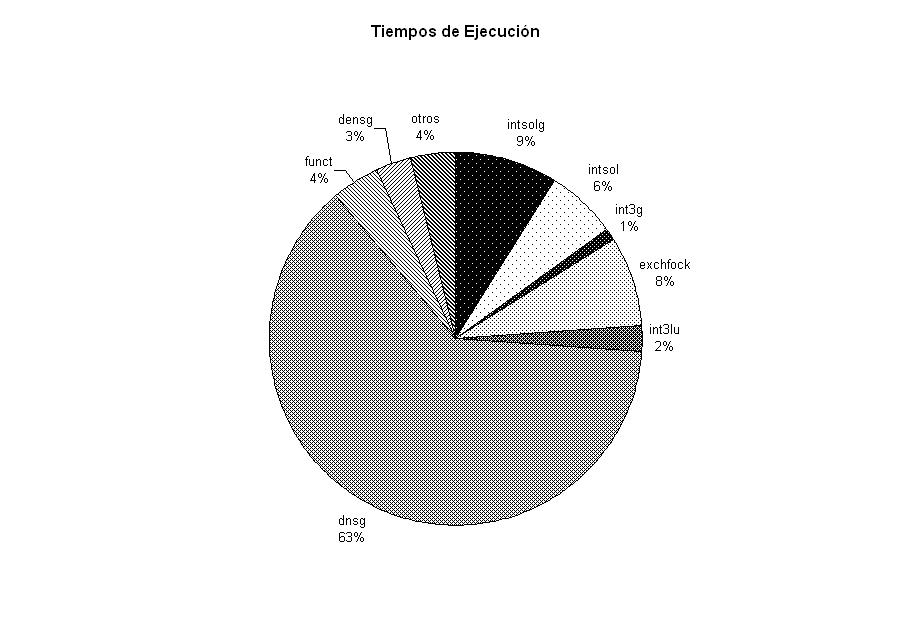
\includegraphics[keepaspectratio, width=14cm]{Profiling2}
\end{center}
\caption[Porcentajes de tiempo consumidos por las rutinas]{\small{Porcentajes de tiempo consumidos por las rutinas.}}
\label{fig:Profiling}
\end{figure}

Con estos resultados pudimos identificar cu\'ales eran las rutinas que conven\'ia analizar para evaluar su posible paralelizaci\'on.

Se puede observar en la figura \ref{fig:Profiling} que si bien la rutina \textsf{dnsg} insume un 62.5\% del tiempo de procesamiento total, esto se debe a la cantidad de veces que es invocada, ya que en cada invocaci\'on su tiempo de procesamieto es casi cero, es decir despreciable respecto de otras.
Lo mismo ocurre con las rutinas \textsf{exchfock}, {\textsf{funct} y \textsf{densg}.

Siguiendo con los resultados del profiling realizado, se buscaron las llamadas correspondientes a las rutinas que calculan la densidad electr\'onica ya que las mismas en las corridas son las que insumen mayor cantidad de tiempo de procesamiento.
Al realizar esta b\'usqueda se encontraron las rutinas \textsf{exchfock}, \textsf{exhnum}, \textsf{exhnumop}, \textsf{exchnum2} y \textsf{exchnum2op}.

Es en estas cinco \'ultimas rutinas es en las que se centra nuestro an\'alisis de paralelizaci\'on.
Se podr\'a observar m\'as adelante que las cinco efect\'uan el mismo tipo de c\'alculo, variando s\'olo en algunos detalles internos como ser utilizaci\'on o no de una matriz resultado, o la cantidad de par\'ametros de salida que tienen.

\section{Implementaci\'on}

La paralelizaci\'on del programa paralelo fue realizada mediante la t\'ecnica de caja negra. Esta t\'ecnica se refiere a ver un sistema en t\'erminos de sus caracter\'isticas de entradas y salidas sin tener en cuenta los procesos intermedios. Esto quiere decir que se analiza el algoritmo en t\'erminos de lo que recibe y entrega.

En primera instancia se reorganiz\'o el c\'odigo de manera de eliminar vicios de programaci\'on y lograr evitar ciertos problemas que pueden traer aparejadas algunas reglas de utilizaci\'on del fortran.
Por ejemplo, al utilizar declaraci\'on impl\'icita de variables si el programador declara que las variables que empiecen con letras de la \texttt{A} a la \texttt{H} ser�n del tipo \texttt{REAL*8} pero luego ante un descuido declara otra variable \texttt{INTEGER} con alg\'un nombre que empiece entre esas letras podr\'an darse errores o diferencias en los resultados.
En etapas posteriores se fueron eliminando las declaraciones impl\'icitas de variables y se constat\'o mediante un $dump$ del estado del programa que no se hubiera modificado nada respecto a la versi\'on serial.

La paralelizaci\'on del algoritmo se realiza a trav\'es de la descomposici\'on del dominio de la integral.

Cada uno de los procesos participantes, tiene en memoria el dominio completo y realiza sobre el subdominio correpondiente sus c\'alculos en forma local.
Finalmente, como es necesario para las operaciones subsiguientes contar con el total de los datos, se realiza la sincronizaci\'on con todos los procesos.

Como se mencion\'o con anterioridad al realizar el profiling se observ\'o que entre un 65\% y 75\% del tiempo era consumido por las rutinas de tipo \textsf{densg} que son las encargadas de calcular los gradientes necesarios para obtener el valor en cada punto de la grilla de trabajo.

Esta rutinas en s\'i consumen muy poco tiempo de ejecuci\'on, pero el problema es que son llamadas en el orden de los millones de veces.

Por este motivo, se buscaron las rutinas desde donde \textsf{dnsg}(y las otras rutinas similares) eran llamadas.
Esto ocurre en las funciones de tipo \textsf{exch}(\textsf{exchfock}, \textsf{exchnum}, \textsf{exchnum2}, \textsf{exchnum2op}).
En las mismas se observ\'o que las llamadas se encontraban dentro de tres ciclos, con los cuales se armaban los puntos de la grilla para cada \'atomo del sistema.

Se decidi\'o paralelizar el algoritmo por el ciclo m\'as externo, que justamente es el que itera por cada \'atomo, para evitar sobrecarga de comunicaci\'on entre los nodos.

En este caso, si el n\'umero de procesos utilizados es menor o igual que el n\'umero de \'atomos con los que se trabaja se dividen los mismos de manera uniforme.
En cambio, si hay m\'as procesos que \'atomos, todo el procesamiento va a un solo nodo, lo cual produce p\'erdidas con respecto al modelo original por la introducci\'on de instrucciones de la librer\'ia $MPI$, operaciones que no son utilizadas a ning\'un fin pr\'actico con un solo proceso(como ser inicializaci\'on de acumuladores) y la inicializaci\'on del sistema paralelo.

En figura \ref{fig:Paralelo} se muestra como se paraleliza el sistema en caso de tener 7 una entrada con 7 \'atomos y dos procesos paralelos.

\begin{figure}[ht!]
\begin{center}
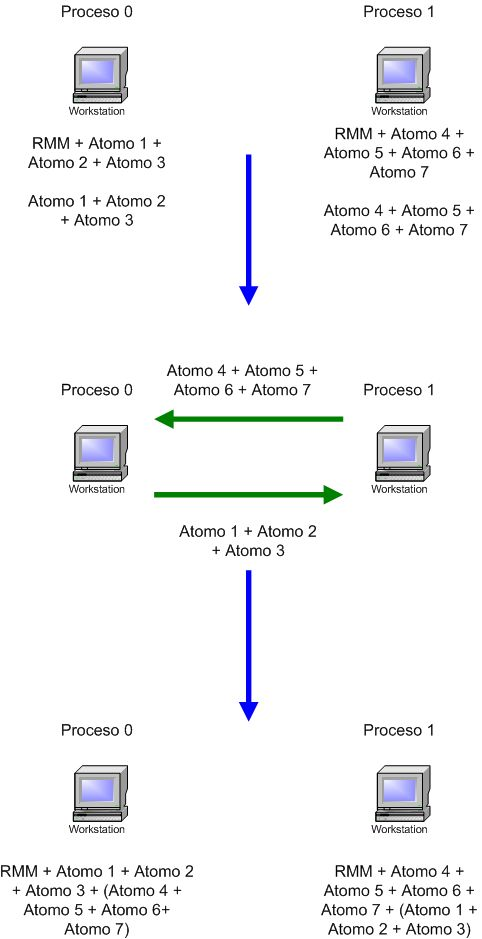
\includegraphics[keepaspectratio, width=10cm]{EjecucionParalela1}
\end{center}
\caption[Forma en que es paralelizado el dominio de 7 \'atomos en dos procesos]{\small{Forma en que es paralelizado el dominio de 7 \'atomos en dos procesos.}}
\label{fig:Paralelo}
\end{figure}

En la figura se ve como en vez de realizar la sumatoria del vector RMM original m\'as los siete \'atomos se toman dos conjuntos. se realizan las sumatorias parciales y luego se suman los resultados para obetener el valor final. Se puede observar que por un lado se hacen las sumatorias parciales, por ejemplo en el proceso 0 se suman RMM m\'as los tres primeros \'atomos y por otro lado en un acumulador se guarda solamente la sumatoria de los \'atomos. Esto es as\'i para poder luego enviar el contenido de los acumuladores a los otros procesos y que RMM no sea sumado $N$ veces con $N$ igual al n\'umero de procesos, sino una \'unica vez.

En cuanto a las modificaciones realizadas al sistema, en el archivo \textsf{main.f} se agregaron sentencias de MPI \cite{Pach96, mpich-install},  para la inicializaci\'on y finalizaci\'on de la utilizaci\'on de la librer\'ia que lo implementa. Se utilizaron las librer\'ias \textsf{MPICH}\cite{MPICH} y \textsf{LAM MPI}\cite{LAM_MPI} para las pruebas realizadas.

En cada uno de los archivos \textsf{exch} se agregaron instrucciones para calcular el n\'umero de procesadores a utilizar de acuerdo a los \'atomos presentes en el sistema, y otras para compartir los resultados parciales obtenidos con el resto de los procesos para luego poder construir el resultado final.

Las llamadas a rutinas de salida debieron ser eliminadas para los procesos distintos al \emph{root} para que el mismo fuera el \'unico en realizar la escritura de datos de salida. Esto fue realizado incluyendo rutinas de \texttt{MPI} en todas las subrutinas que realizaban actividades de I/O para poder preguntar que n\'umero de proceso era sobre el que se corr\'ian estas rutinas. En caso de que el proceso fuera distintos del \emph{root} (proceso 0) no se ejecutan las instrucciones de entrada/salida.

\section{Problemas surgidos durante la implementaci\'on}%


Uno de los primeros problemas surgidos durante la implementaci\'on del software paralelo fu\'e la configuraci\'on del sistema MPI bajo Fortran. En el archivo main.f se agregaron las instrucciones de inicializaci\'on de MPI, sin embargo en las subrutinas del sistema las contantes definidas en la librer\'ia \texttt{MPIF} no eran reconocidas, lo cu\'al produc\'ia errores al ejecutar el software.

Un ejemplo de este caso se produjo con el comunicador \texttt{MPI\_COMM\_WORLD}que incluye a todos los procesos ejecutandose en MPI. Al no ser reconocido este comunicador no hab\'ia forma de enviar y recibir mensajes entre procesos lo cu\'al produc\'ia un aborto del sistema. Esta situaci\'on luego de ser investigada en un primer momento se solucion\'o pasando el comunicador como par\'ametro a todas las rutinas que pudieran llegar a utilizarlo. Luego, se descubri\'o que el sistema reconoc\'ia al valor 91 (\texttt{MPI\_COMM\_WORLD}) como variable global pero no as\'i a su nombre de alias. Por lo tanto se quitaron los pasajes del comunicador como par\'ametro y se utilizaron directamente los valores integer correspondientes.

Ocurrieron problemas similares con otro tipo de constantes definidas en \texttt{MPIF} pero una vez encontrado el error fue simple solucionarlo en situaciones posteriores. Finalmente el problema fue solucionado incluyendo la sentencia de pre-procesamiento \texttt{include mpif.h} en todos los archivos donde se utilizan instrucciones de \texttt{MPI}.
De esta forma el compilador reconoci\'o todas las constantes con sus alias y no fue necesario utilizar los integer correspondientes.

El motivo por el cual se opt\'o por incluir la sentencia de pre-procesamiento \texttt{include mpif.h} (que aunque parezca una instrucci\'on corta lo que hace es en momento de compilaci\'on "pegar" el contenido de \texttt{mpif.h} en lugar de la sentencia) en vez de continuar utilizando los integer correspondientes es por la portabilidad del programa. Distintos proveedores de implementaciones de librer\'ias \texttt{MPI} como ser \texttt{MPICH}\cite{MPICH} o \texttt{LAM}\cite{LAM_MPI} le asignan distintos valores a las constantes, por lo cual en caso de pasar de uno a otro en vez de utilizar el alias y reemplazarlo por el valor correspondiente automaticamente el compilador, uno deber\'ia recorrer todo el c\'odigo poniendo el n\'umero correcto, lo cual no solo no es pr\'actico sino que es una pr\'actica aberrante de programaci\'on que no deber\'ia ocurrir.

Otro problema surgido fue con el pasaje de resultados mediante mensajes al proceso \emph{root}(el proceso 0) para que el mismo contin\'ue realizando los c\'alculos pertinentes. En los archivos modificados se deben pasar vectores al proceso root para que el mismo contin\'ue con los c\'alculos y luego el mismo debe enviar tambi\'en vectors con informaci\'on al resto de los procesos. Sin embargo, en una primera instancia no se lograba pasar un vector completo mediante directivas Send/Receive por lo cual se enviaba por mensajes de a un elemento del vector por vez. Est\'o estaba lejos de ser lo \'optimo debido al overhead generado por el env\'io de mensajes. Se comprob\'o que el problema se debi\'a a una mala configuraci\'on y utilizaci\'on de $MPICH$ y finalmente se lograron pasar los vectores en forma completa.

Por otra parte, en busca de una alta performance del programa, se buscaron diversas formas de realizar el intercambio de informaci\'on entre procesos. Como se mencion\'o con anterioridad la primera implementaci\'on inclu\'ia el env\'io de cada uno de los valores pertenecientes a los vectores por forma separada mediante mensajes bloqueantes utilizando el par Send/Receive. Esto produc\'ia un overhead que produc\'ia que el tiempo del sistema paralelo excediera por mucho los tiempos del serial. Luego se lograron mandar los vectores completos por medio de las mismas instrucciones, lo cual redujo los tiempos de ejecuci\'on, pero a\'un as\'i debido a la cantidad de procesos, y topolog\'ias formadas con los mismos para el env\'io de mensajes, la performance estaba lejos de los esperado. Finalmente se utilizaron instrucciones de comunicaci\'on colectivas para reducir los tiempos de comunicaci\'on. Fueron utilizadas las instrucciones $MPI\_Bcast$ y $MPI\_Allreduce$

La instruccion $MPI\_Bcast$ realiza una comunicaci\'on colectiva donde un proceso env\'ia los mismos datos a todos los procesos presentes en el comunicador. De acuerdo a la cantidad de procesos presentes en el comunicador $MPI$ optimiza el env\'io de acuerdo a la topolog\'ia que puede haber. Por ejemplo, puede env\'iar los mensajes con una topolog\'ia de \'arbol binario, lo cual reduce el tiempo de env\'io de lineal a logar\'itmico. Lo mismo sucede con la instrucci\'on $MPI\_Allreduce$, que genera una topolog\'ia especial entre procesos para realizar una operaci\'on determinada entre t\'erminos que est\'an presentes en cada uno de los procesos, y deja el resultado de la operaci\'on presente en todos los procesos del comunicador. Esto permite por ejemplo que si los t''erminos de una sumatoria est\'an repartidos entre todos los procesos, por medio de esta instrucci\'on se le puede indicar a $MPI$ que realice la sumatoria y deje el resultado en todos los procesos en una variable de destino. Estas instrucciones se comportan en forma mucho m\'as eficiente que si uno realizara las mismas operaciones por medio de pares Send/Receive.

Por medio de la comunicaci\'on colectiva se logr\'o bajar considerablemente el tiempo de ejecuci\'on de manera de que la performance del programa paralelo fuese mejor que la del serial, lo cual era el objetivo de este trabajo. Los resultados se ver\'an m\'as adelante en la secci\'on correspondiente.

Por \'ultimo, cuando se cre\'ia que se hab\'ia logrado el objetivo de desarrollar un programa paralelo que se comportase de manera similar al serial pero con una mejor performance, se tuvo un problema que fue determinante en la realizaci\'on de este trabajo. El mismo surgi\'o cuando se observ\'o que los resultados obtenidos en la matriz $RMM$ utilizada para calcular la integral difer\'ian en el programa paralelo con respecto al serial. Esto pudo ser observado gracias a la realizaci\'on de una rutina en lenguaje de programaci\'on Fortran 77 desarrollada para este trabajo que permite guardar en memoria(mediante un archivo de texto) una cantidad de variables que cre\'imos convenientes analizar para determinar la correctitud de los c\'alculos.

En un principio se pens\'o que el problema ser\'ia debido a un error en la manera de calcular el mismo, pero luego de un an\'alisis se confirm\'o que el c\'alculo era correcto. Para tal efecto se fueron guardando los diversos t\'erminos participantes en las sumatorias y los mismos fueron sumados "a mano".
A partir de la confirmaci\'on de la correctitud de c\'alculo se intuy\'o que el problema podr\'ia corresponder al redondeo realizado sobre n\'umeros de punto flotante, debido a que la diferencia era de unos pocos decimales muy peque\~nos.
Para corroborar si el problema era de redondeo se realizaron una bater\'ia de tests.
En todos los casos de test se utiliz\'o un entorno con 4 \'atomos.

\begin{itemize}
\item Se corri\'o el algoritmo serial y el paralelo y se realiz\'o una comparaci\'on entre los estados guardados por ambos. As\'i se detect\'o una inconsistencia en los valores del vector RMM.
\item Se guardaron los valores de RMM calculados por el algoritmo serial pero separados en los atomos 1-2 y 3-4. O sea, inicialmente se calcularon con el programa serial las primeras dos iteraciones. Luego se realiz\'o la corrida con los 4 \'atomos pero solo guardando el resultado de las iteraciones 3 y 4.
\item Se guard\'o el estado calculado por el algoritmo paralelo (corrido en 2 procesos) correspondiente al proceso 0 que calcula los atomos 1-2 y al proceso 1 que calcula 3-4.
\item Se compararon los resultados correspondientes y se observ\'o que los calculos de RMM eran iguales.
\end{itemize}

De esta manera se concluy\'o que el problema radicaba en la uni\'on de los resultados obtenidos en los distintos procesos del programa paralelo.

Una vez reducido el \'area donde pod\'ia ocurrir el problema se procedieron a realizar otros tests para determinar finalmente el problema. Para tal efecto se realiz\'o una modificacion al programa serial para que calcule en RMM el resultado de las 2 primeras iteraciones, y las \'ultimas dos las guarde en un acumulador. Finalmente se uni\'o el vector RMM con el acumulador por medio de sumas. Esto hizo que el programa serial diera el mismo resultado que el paralelo. De esta manera se demostr\'o que el problema se debe a la limitaci\'on generada por la finitud de los n\'umeros representados en la computadora, lo cual es un problema ampliamente conocido en los m\'etodos num\'ericos.

\subsection{Errores de punto flotante surgidos durante la implementaci\'on}%

En el mundo matem\'atico tradicional puede haber n\'umeros con una cantidad infinita de d\'igitos no peri\'odicos. La aritm\'etica que empleamos en este mundo define $\sqrt(3)$ como el \'unico n\'umero positivo que cuando se multiplica por s\'i mismo produce el entero 3. Sin embargo, en el mundo de la computaci\'on todo n\'umero representable tiene s\'olo un n\'umero fijo y finito de d\'igitos. Puesto que $\sqrt(3)$ no tiene una representaci\'on de d\'igitos finitos, en el interior de la computadora se le da una representaci\'on aproximada cuyo cuadrado no ser\'a exactamente 3, aunque con toda probabilidad estar\'a lo bastante cerca al 3 para resultar aceptable en la generalidad de los casos. Casi siempre la representaci\'on y aritm\'etica computacionales son satisfactorias
y pasan inadvertidas o sin problemas. Pero no siempre es as\'i, y en este caso la diferencia producida es amplificada de forma tal de que finalmente el resultado obtenido sea inutilizable\cite{Burden}.

El error de redondeo se da cuando usamos una calculadora o computadora para efectuar c\'alculos con n\'umeros reales. El error surge porque las operaciones aritm\'eticas realizadas en una m\'aquina incluyen exclusivamente n\'umeros finitos de d\'igitos, de manera que los c\'alculos se llevan a cabo con representaciones aproximadas de los n\'umeros reales. En una computadora com\'un, s\'olo un conjunto relativamente peque\~no de n\'umeros reales se utiliza para representar a todos estos n\'umeros. El subconjunto que contiene \'unicamente n\'umeros racionales, tanto positivos como negativos, y almacena una parte fraccionaria es denominada mantisa, junto con una parte exponencial conocida con el nombre de caracter\'istica. La composici\'on de un n\'umero de punto flotante seg\'un el IEEE es un d\'igito binario para el signo, ocho d\'igitos para el exponente y 23 para la mantisa. Un n\'umero de doblre precisi\'on (como los utilizados para los nuestros c\'alculos) est\'a compuesto por un d\'igito para le signo, once para el exponente y 52 para la mantisa.

No solo la representaci\'on de los n\'umeros es poco exacta, la aritm\'etica efectuada en una computadora tambi\'en lo es. Esta aritm\'etica requiere el manejo de los d\'igitos binarios con varias operaciones l\'ogicas o de traslaci\'on. Si una representaci\'on o c\'alculo con d\'igitos finitos introduce un error, \'este crece a\'un m\'as cuando lo dividimos entre un n\'umero de peque\~na magnitud (o equivalentemente multiplicando por un n''umero de gran magnitud).


\section{Resoluci\'ones a los errores de punto flotante en la implementaci\'on}

Se plantear\'an en esta secci\'on dos soluciones ampliamente conocidas para solucionar el tipo de problema presentado. Luego en la secci\'on de resultados y discusi\'on se explicar\'a porque la primera soluci\'on presentada no result\'o satisfactoria.

\subsection{Ampliaci\'on de la precisi\'on}

Para solucionar los problemas de precisi\'on en punto flotante inicialmente se opt\'o por duplicar el tama\~no de las variables que presentaban este inconveniente en la implementaci\'on.
Para realizar esto se opt\'o por cambiar de compilador ya que los compiladores de Fortran 77 no aceptan n\'umeros de punto flotante cuadruples (llamados long double o Real*16 seg\'un el lenguaje utilizado). Por esto es que se migr\'o todo el programa de manera de que pueda ser compilado mediante el Intel Fortran Compiler para Linux.
Esta migraci\'on acarre\'o los inconvenientes que cualquier traspaso de un lenguaje a otro puede acarrear, debido a que los chequeos realizados por los compiladores modernos suelen ser m\'as exigentes que los antiguos.
Luego de sortear los inconvenientes de migraci\'on surgi\'o la necesidad de obtener y utilizar una librer\'ia de Message Passing que permita el env\'io y recepci\'on de datos de tipo Real*16.
Ninguna librer\'ia de las investigadas (Intel, LAM, MPICH) ten\'ia implementado este tipo de datos para Fortran. Sin embargo, la librer\'ia MPICH ten\'ia implementado el tipo long double para el lenguaje de programaci\'on C/C++.
El inconveniente surgido es que en las m\'aquinas IAS-32 y AMD comunes ese tipo de datos es de 80 bits y no de 128 como en realidad es el tipo REAL*16.
Finalmente, se opt\'o por utilizar el tipo correspondiente a long double de MPICH coriendolo en una m\'aquina SMP Xeon Dual, Papita, la cual fue cedida por Intel Argentina, AMD Opteron e Itanium ya que en las mismas este tipo de dato y el Real*16 son equivalentes (128 bits).
Se realizaron diversas pruebas para corroborar que luego de esta soluci\'on al problema de punto flotante la diferencia entre los resultados del programa serial y el paralelo no eran significativos.

\subsection{Reordenamiento del C\'alculo}

Para resolver finalmente el problema de precisi\'on en punto flotante se intent\'o realizar un reordenamiento de los c\'alculos para realizar la sumatoria de forma tal que la p\'erdida de informaci\'on en la misma fuera similar a la que ocurre en el programa original.

Para realizar esta soluci\'on se debieron hacer diversos an\'alisis. En primera instancia se observaron los exponentes de los t\'erminos participantes en la sumatoria a realizar. Para realizar esto se modific\'o el programa para guardar en archivos cada uno de los vectores participantes en la sumatoria. Luego estos archivos fueron importados en una planilla de c\'alculo para poder observarlos en conjunto.
A continuaci\'on se realiz\'o una clasificaci\'on de los datos de acuerdo a los exponentes de los mismos, categoriz\'andolos entre $E-50$ y $E+04$. Por otro lado fueron separados los ceros absolutos, ya que de otra forma contar\'ian dentro de la categor\'ia $E+00$ lo cual es incorrecto. Este an\'alisis nos permiti\'o conocer la distribuci\'on aproximada de los datos con los que se estaba trabajando.

Inicialmente, la idea planteada era reducir la p\'erdida de d\'igitos significativos en la operatoria, suponiendo que de esa manera el sistema se iba a estabilizar arrojando resultados similares a los generados por el programa original. De esta manera fu\'e que se pens\'o en ordenar las sumatorias de forma tal que los t\'erminos se sumen de menor a mayor para minimizar la p\'erdida. Sin embargo, esta posibilidad fue desechada ya que al alterar el orden de la suma, como el programa era tan inestable num\'ericamente hablando, los resultados obtenidos no eran los esperados.

Por estos motivos se pens\'o otra soluci\'on, analizar las p\'erdidas ocasionadas en cada operaci\'on del sistema serial de manera de intentar reproducir las mismas de la forma m\'as precisa posible en el programa paralelo.

Con este objetivo en mente el primer an\'alisis realizado fu\'e hallar la diferencia absoluta entre los exponentes de los t\'erminos de cada suma realizada, tanto en el programa serial como en el paralelo.
De esta forma fu\'e realizada una planilla en donde si se sumaban por ejemplo un n\'umero con exponente $E-10$ y otro con $E-05$, se anotaba una p\'erdida de cinco posiciones, ya que el resultado tendr\'a por lo menos exponente $E-05$. Uno de los aspectos a tener en cuenta nuevamente, fue la inclusi\'on de ceros en la planilla. La diferencia entre un cero y cualquier otro n\'umero al momento de realizar la sumatoria es nula, porque no se pierden d\'igitos como si ocurre entre dos n\'umeros distintos de cero con diferentes exponentes. Los ceros poseen exponentes $E+00$ por lo cual debieron ser diferenciados de los valores distintos a cero con igual exponente para no cometer errores en los c\'alculos.

Luego de obtener estos datos se analizaron las distribuciones de estas p\'erdidas para poder observar de forma gr\'afica cual era el problema que se planteaba.

Suponiendo finalmente que los d\'igitos significativos en nuestros c\'alculos fueran siete, se realiz\'o un an\'alisis de cuales eran las operaciones en las cuales se perd\'ian menos de 7 d\'igitos y en cuales m\'as y finalmente se grafic\'o las dispersi\'on de estos datos.

\begin{figure}[ht!]
\begin{center}
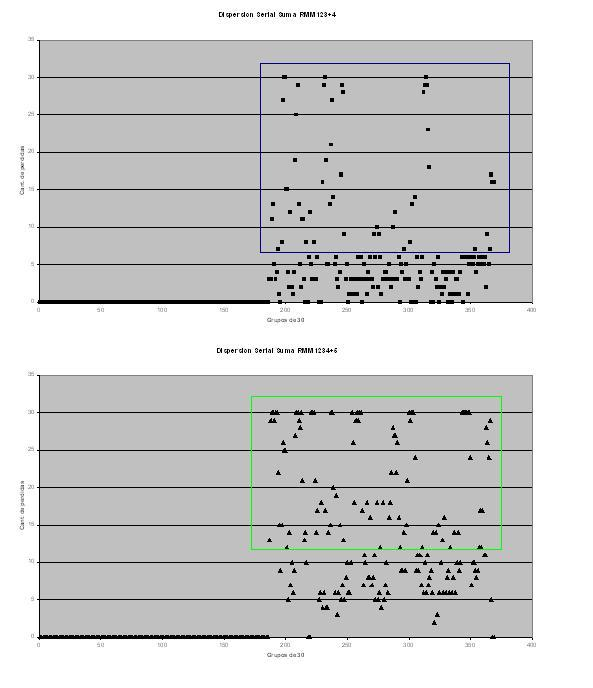
\includegraphics[keepaspectratio, width=14cm]{DispersionSerial1}
\end{center}
\caption[Dispersi\'on de p\'erdida de d\'igitos significativos en la cuarta y quinta suma del algoritmo serial]{\small{Dispersi\'on de p\'erdida de d\'igitos significativos en la cuarta y quinta suma del algoritmo serial.}}
\label{fig:DispersionSerial1}
\end{figure}

\begin{figure}[ht!]
\begin{center}
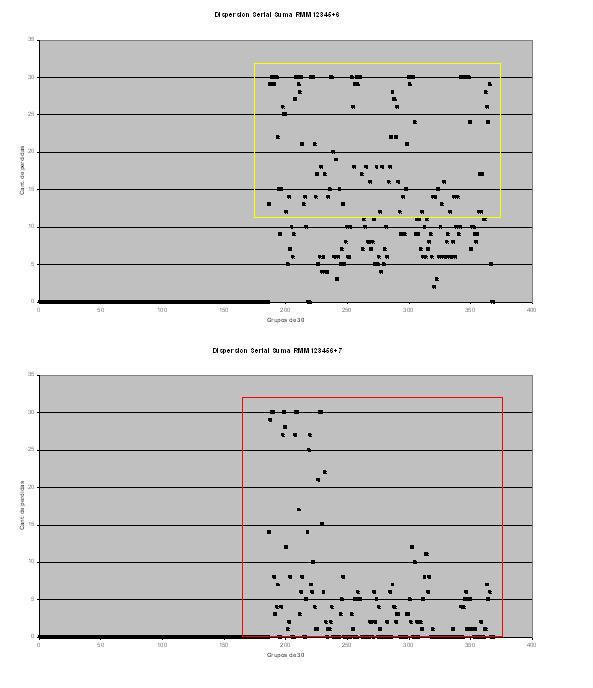
\includegraphics[keepaspectratio, width=14cm]{DispersionSerial2}
\end{center}
\caption[Dispersi\'on de p\'erdida de d\'igitos significativos en la sexta y septima suma del algoritmo serial]{\small{Dispersi\'on de p\'erdida de d\'igitos significativos en la sexta y septima suma del algoritmo serial.}}
\label{fig:DispersionSerial2}
\end{figure}

\begin{figure}[ht!]
\begin{center}
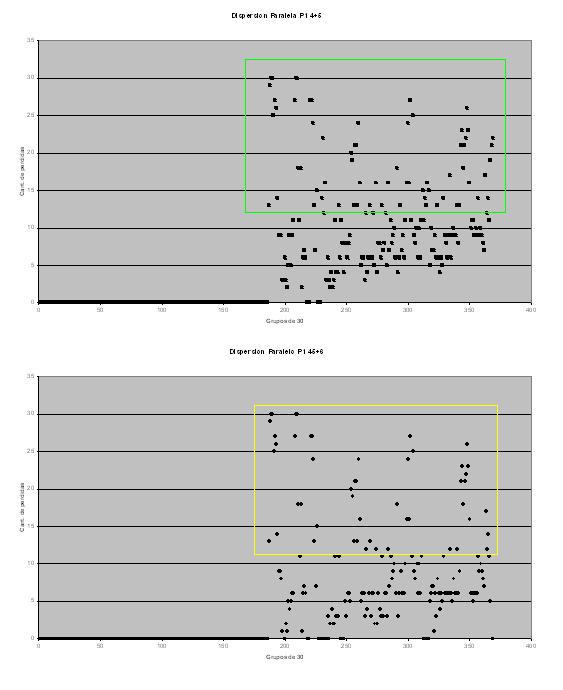
\includegraphics[keepaspectratio, width=14cm]{DispersionParalelo1}
\end{center}
\caption[Dispersi\'on de p\'erdida de d\'igitos significativos en las dos primeras sumas del proceso 1 del algoritmo paralelo]{\small{Dispersi\'on de p\'erdida de d\'igitos significativos en las dos primeras sumas del proceso 1 del algoritmo paralelo.}}
\label{fig:DispersionParalelo1}
\end{figure}

\begin{figure}[ht!]
\begin{center}
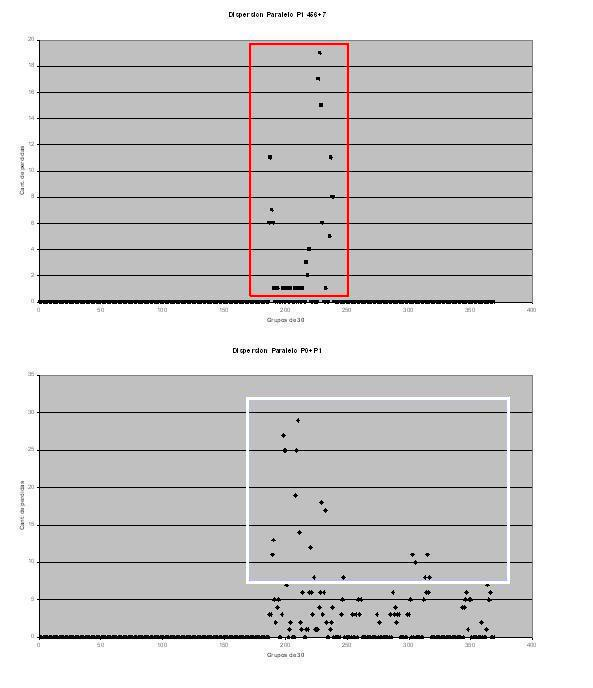
\includegraphics[keepaspectratio, width=14cm]{DispersionParalelo2}
\end{center}
\caption[Dispersi\'on de p\'erdida de d\'igitos significativos en la tercera suma del proceso 1 del algoritmo paralelo y la posterior uni\'on de los dos procesos]{\small{Dispersi\'on de p\'erdida de d\'igitos significativos en la tercera suma del proceso 1 del algoritmo paralelo y la posterior uni\'on de los dos procesos.}}
\label{fig:DispersionParalelo2}
\end{figure}

No fueron graficados los resultados tanto del proceso 0 como las primeras tres sumatorias del sistema serial debido a que estos datos eran id\'enticos(y as\'i se supn\'ia que deb\'ia ser). Los datos de las figuras \ref{fig:DispersionSerial1} y \ref{fig:DispersionSerial2} correponden a las sumatorias del programa serial (RMM123+4, RMM1234+5, RMM12345+6 y RMM123456+7 respectivamente) y los de las figuras \ref{fig:DispersionParalelo1} y \ref{fig:DispersionParalelo2} al paralelo(4+5, 45+6, 456+7 y Proceso0+4567 respectivamente), donde cada n\'umero indica los valores del \'atomo correspondiente (1 es \'atomo 1, y as\'i sucesivamente).

Puede observarse que hay una cierta cantidad de datos en el programa paralelo que no son p\'erdidos y en el serial s\'i. Esto se debe principalmente a que en el proceso 1 la diferencia con los resultados parciales no son tan grandes con respecto a los nuevos valores que se van sumando como para que se produzcan tales p\'erdidas. Observando los datos se vi\'o que la mayor diferencia se daba generalmente contra el valor inicial de RMM, que en muchas ocasiones pose\'ia un valor mayor al de los \'atomos que se suman posteriormente.

Finalmente de la observaci\'on de los datos se lleg\'o a una soluci\'on alternativa al problema. Si bien los resultados obtenidos no eran iguales a los del serial, los mismos eran muy similares, y a los efectos de la investigaci\'on qu\'imica para la cual se utilizar\'ian, eran v\'alidos.

La soluci\'on implementada consisti\'o en agregar en cada uno de los procesos un valor determinado de forma tal que en cada sumatoria se ocasione una p\'erdida similar a la ocurrida en el programa serial, y luego finalmente restarle ese valor al total. Por ejemplo, si en el programa serial se realizaba una suma entre el vector RMM original m\'as los \'atomos del 1 al 7, en el paralelo se suma por un lado el vector RMM m\'as los \'atomos 1,2 y 3 y en el otro, aunque deber\'ian sumarse s\'olo los \'atomos 4 a 7, se le agrega un valor inicial que luego es finalmente restado antes de unir ambos procesos.

Al analizar como eran los valores utilizados en las operaciones se observ\'o que la mayor parte de las p\'erdidas se daban debido a la diferencia de magnitud entre los valores del vector original RMM y el resto de los \'atomos como se mencion\'o con anterioridad. Esto quiere decir que en una gran cantidad de casos en el sistema serial al momento de sumar el cuarto \'atomo el orden de magnitud presentado por la sumatoria de RMM m\'as el resto de los \'atomos correspondientes al proceso era igual al del RMM original. Por este motivo se opt\'o por tomar el RMM original como n\'umero a sumar y restar en todos los procesos para producir la p\'erdida de informaci\'on necesaria.

Esta nueva soluci\'on puede observarse en la figura \ref{fig:EjecucionParalela2}

\begin{figure}[ht!]
\begin{center}
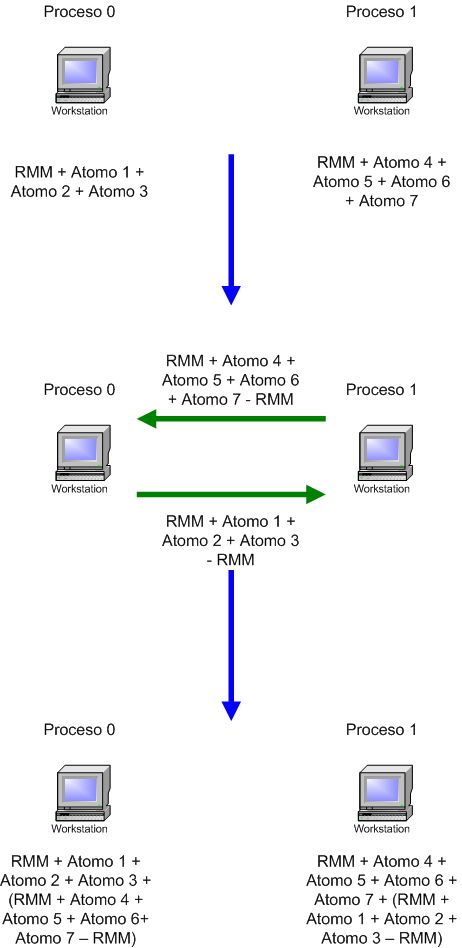
\includegraphics[keepaspectratio, width=10cm]{EjecucionParalela2}
\end{center}
\caption[Forma en que es paralelizado el dominio de 7 \'atomos en dos procesos con reordenamiento de c\'alculo]{\small{Forma en que es paralelizado el dominio de 7 \'atomos en dos procesos con reordenamiento de c\'alculo.}}
\label{fig:EjecucionParalela2}
\end{figure}

Finalmente se realizaron diversas corridas para corroborar el buen funcionamiento de esta implementaci\'on y se obtuvieron los resultados que se ver\'an en la proxima secci\'on, Resultados y Discusi\'on.


\pagebreak
\chapter{Resultados y Discusi\'on}

\textbf{La entrada de 7 \'atomos es un peroxinitrito (OONO) m\'as un di\'oxido de carbono (CO2) cu\'anticos m\'as 498 mol\'eculas de agua}

\textbf{La entrada de 4 \'atomos es s\'olo el peroxinitrito con las 498 mol\'eculas de agua}

Una vez realizadas implementado el algoritmo con precisi\'on exendida se realizaron corridas en una m\'aquina SMP Xeon Dual, obteni\'endose los resultados de la tabla \ref{tab:TiemposEjecucion1}.
La misma puede observarse de mejor manera en la figura \ref{fig:Papita128}. Se utiliz\'o la entrada de 7 \'atomos variando la cantidad de pasos a realizarse.


\begin{table}
\begin{center}
\begin{tabular}{|c|c|c|c|}
\hline
\ & \textbf{100 pasos}& \textbf{500 pasos}& \textbf{1000 pasos}\\
\hline
\texttt{Serial} & 24:10 & 128:25 & 251:52 \\
\texttt{Paralelo}  & 22:35 & 107:00 & 215:55 \\
\hline
\end{tabular}
\end{center}
\caption[Tiempos de ejecuci\'on en m\'aquina SMP Xeon Dual con 128 bits de precisi\'on]{\small{Tiempos de ejecuci\'on total del programa en una m\'aquina SMP Xeon Dual con 7 \'atomos con 128 bits de precisi\'on. Los resultados est\'an expresados en HH:MM.}}
\label{tab:TiemposEjecucion1}
\end{table}


\begin{figure}[ht!]
\begin{center}
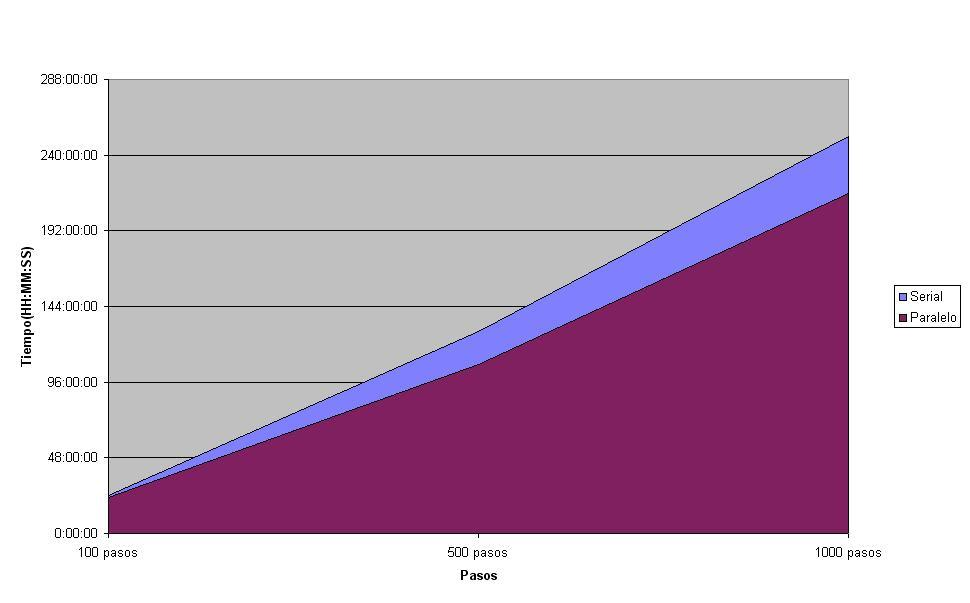
\includegraphics[keepaspectratio, width=14cm]{Papita128}
\end{center}
\caption[Tiempos de ejecuci\'on en m\'aquina SMP]{\small{Tiempos de ejecuci\'on total del programa en una m\'aquina SMP Xeon Dual con 7 \'atomos. Los resultados est\'an expresados en HH:MM.}}
\label{fig:Papita128}
\end{figure}

A pesar de que puede observarse c\'omo una vez realizada la transformaci\'on de datos de tipo $REAL*8$ a $REAL*16$ el programa paralelo logra una mejora de casi un 15\% con respecto al serial esta soluci\'on no es v\'alida. \'Esto es as\'i debido a que el programa serial modificado tarda un orden de magnitud m\'as que el original. Las causas de este comportamiento es debido a que no existe a\'un una maquina en el mercado que trabaje en forma nativa con n\'umeros de 128 bits. Tanto la SMP Xeon Dual como las Itanium de Intel, y las Opteron de AMD realizan una emulaci\'on, lo cual quiere decir que trabajan con n\'umeros de esa longitud pero trabaj\'andolos con software y no con hardware como s\'i ocurre con los n\'umeros de 64.
Es debido a esta emulaci\'on por software que la velocidad de procesamiento se ve afectada.

Por estos motivos, a pesar de que el programa paralelo funcione mejor que el serial modificado (lo cual podr\'ia indicar que a futuro cuando haya computadoras de 128 bits nativos, la soluci\'on servir\'a), no se logr\'o el objetivo de esta investigaci\'on, por lo cual se opt\'o por proceder con la implementaci\'on de la segunda opci\'on. A continuaci\'on se muestran gr\'aficos de eficiencia, overhead y speedup de este m\'etodo en las figuras \ref{fig:Speedup128}, \ref{fig:Eficiencia128}, \ref{fig:Overhead128} y \ref{fig:OverheadP128} respectivamente.

\begin{figure}[ht!]
\begin{center}
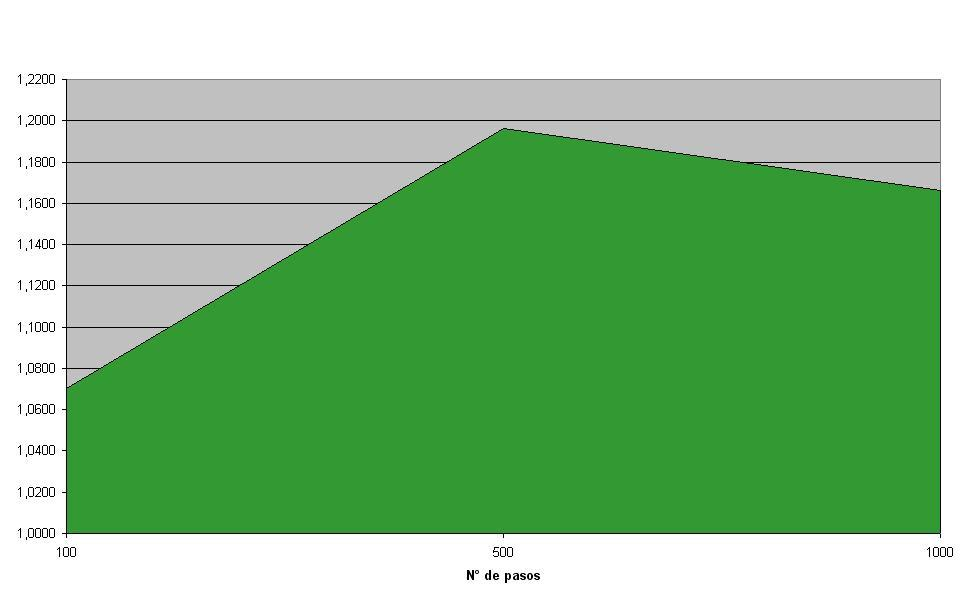
\includegraphics[keepaspectratio, width=14cm]{Speedup128}
\end{center}
\caption[Speedup del programa de 128 bits en 2 procesos.]{\small{Speedup del programa de 128 bits en 2 procesos.}}
\label{fig:Speedup128}
\end{figure}

\begin{figure}[ht!]
\begin{center}
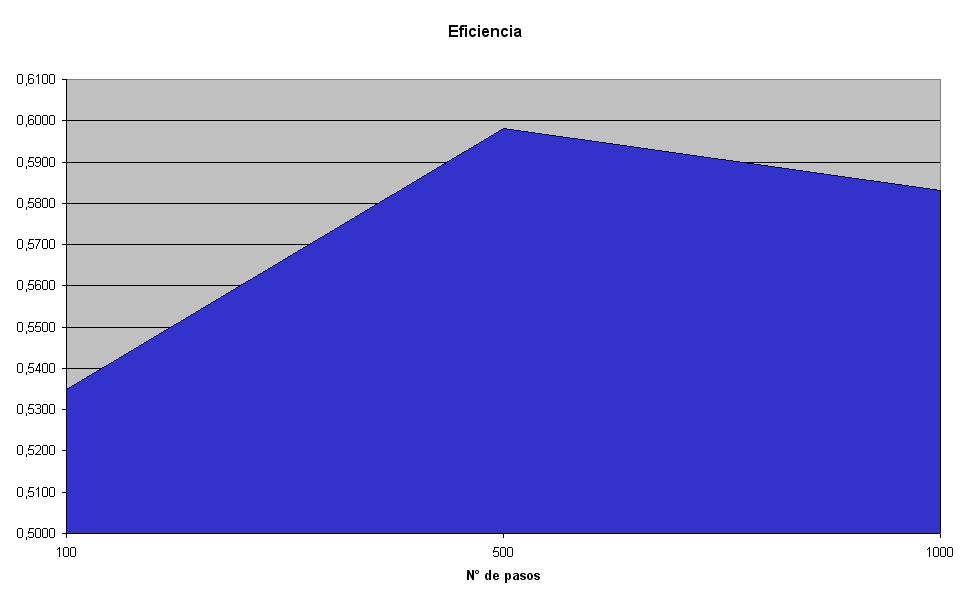
\includegraphics[keepaspectratio, width=14cm]{Eficiencia128}
\end{center}
\caption[Eficiencia del programa de 128 bits en 2 procesos.]{\small{Eficiencia del programa de 128 bits en 2 procesos.}}
\label{fig:Eficiencia128}
\end{figure}

\begin{figure}[ht!]
\begin{center}
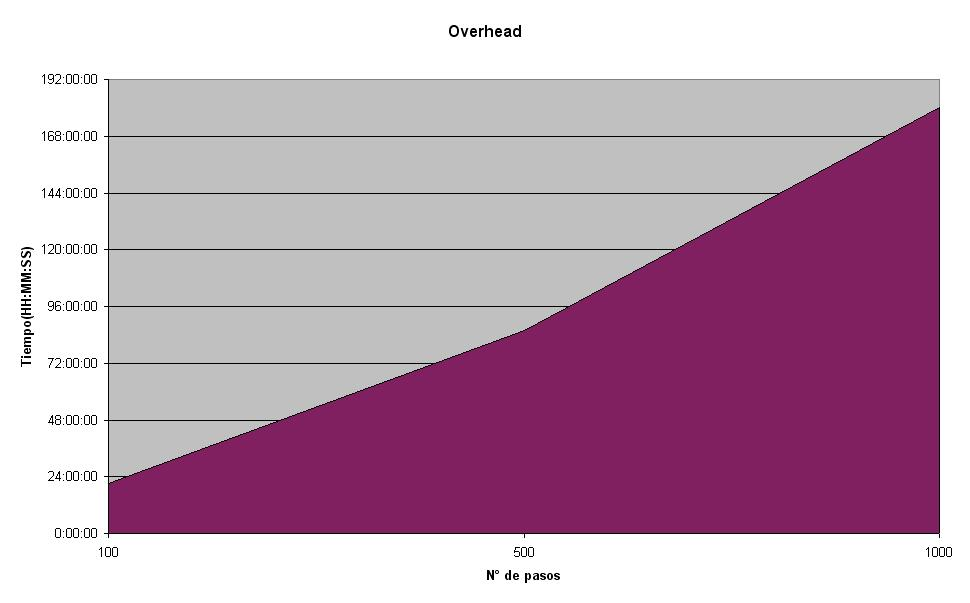
\includegraphics[keepaspectratio, width=14cm]{Overhead128}
\end{center}
\caption[Overhead del programa de 128 bits en 2 procesos.]{\small{Overhead del programa de 128 bits en 2 procesos.}}
\label{fig:Overhead128}
\end{figure}

\begin{figure}[ht!]
\begin{center}
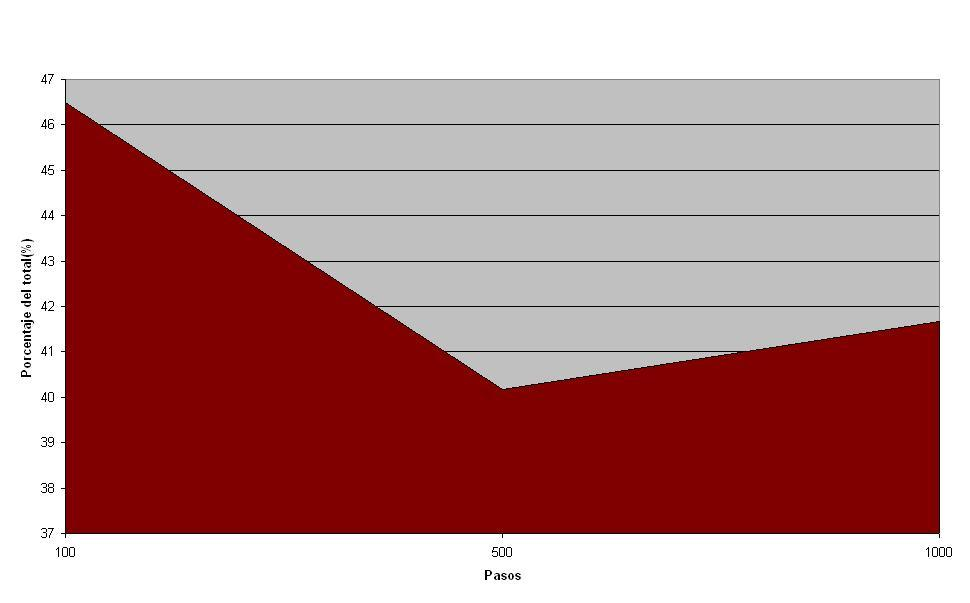
\includegraphics[keepaspectratio, width=14cm]{OverheadP128}
\end{center}
\caption[Overhead del programa de 128 bits en 2 procesos.]{\small{Overhead del programa de 128 bits en 2 procesos.}}
\label{fig:OverheadP128}
\end{figure}

No fueron realizadas corridas con otro tipo de entradas o en otras m\'aquinas con esta versi\'on debido a la limitaci\'on de performance comentada con anterioridad.


En segunda instancia se implement\'o la soluci\'on de reordenamiento de c\'alculo mencionada en la secci\'on anterior. Para esta implementaci\'on inicialmente se realizaron diversas corridas en la m\'aquina SMP Xeon Dual para corroborar que los resultados obtenidos se correspondan a los del programa serial. Estas corridas iniciales fueron realizadas con una entrada de 4 \'atomos y variando la cantidad de pasos de ejecuci\'on. Los tiempos de ejecuci\'on de estas corridas y otros valores de performance pueden observarse en las tablas \ref{tab:Tiempos4Atomos}, \ref{tab:Speedup4Atomos}, \ref{tab:Eficiencia4Atomos} y \ref{tab:Overhead4Atomos}.


\begin{table}
\begin{center}
\begin{tabular}{|c|c|c|c|c|}
\hline
\ & \textbf{100 pasos}& \textbf{200 pasos}& \textbf{300 pasos}& \textbf{400 pasos}\\
\hline
\texttt{Serial} & 14:30 & 29:15 & 43:10 & 58:20 \\
\texttt{Paralelo}  & 11:30 & 22:45 & 34:30 & 45:40 \\
\hline
\end{tabular}
\end{center}
\caption[Tiempos de ejecuci\'on en m\'aquina SMP Xeon Dual con reordenamiento de c\'alculo]{\small{Tiempos de ejecuci\'on total del programa en una m\'aquina SMP Xeon Dual con 4 \'atomos con reordenamiento de c\'alculo en el programa. Los resultados est\'an expresados en MM:SS.}}
\label{tab:Tiempos4Atomos}
\end{table}

\begin{table}
\begin{center}
\begin{tabular}{|c|c|c|c|c|}
\hline
\ & \textbf{100 pasos}& \textbf{200 pasos}& \textbf{300 pasos}& \textbf{400 pasos}\\
\hline
\texttt{Paralelo}  & 1.2608 & 1.2857 & 1.2512 & 1.2773 \\
\hline
\end{tabular}
\end{center}
\caption[Speedup en m\'aquina SMP Xeon Dual con reordenamiento de c\'alculo]{\small{Speedup del programa en una m\'aquina SMP Xeon Dual con 4 \'atomos con reordenamiento de c\'alculo en el programa.}}
\label{tab:Speedup4Atomos}
\end{table}

\begin{table}
\begin{center}
\begin{tabular}{|c|c|c|c|c|}
\hline
\ & \textbf{100 pasos}& \textbf{200 pasos}& \textbf{300 pasos}& \textbf{400 pasos}\\
\hline
\texttt{Paralelo}  & 0.6304 & 0.6428 & 0.6256 & 0.6386 \\
\hline
\end{tabular}
\end{center}
\caption[Eficiencia en m\'aquina SMP Xeon Dual con reordenamiento de c\'alculo]{\small{Eficiencia del programa en una m\'aquina SMP Xeon Dual con 4 \'atomos con reordenamiento de c\'alculo en el programa.}}
\label{tab:Eficiencia4Atomos}
\end{table}

\begin{table}
\begin{center}
\begin{tabular}{|c|c|c|c|c|}
\hline
\ & \textbf{100 pasos}& \textbf{200 pasos}& \textbf{300 pasos}& \textbf{400 pasos}\\
\hline
\texttt{Paralelo}  & 36.95\% & 35.71\% & 37.43\% & 36.13\% \\
\hline
\end{tabular}
\end{center}
\caption[Overhead en m\'aquina SMP Xeon Dual con reordenamiento de c\'alculo]{\small{Overhead del programa en una m\'aquina SMP Xeon Dual con 4 \'atomos con reordenamiento de c\'alculo en el programa.}}
\label{tab:Overhead4Atomos}
\end{table}

Finalmente, una vez verificados los resultados se procedi\'o a realizar corridas m\'as extensas con un problema m\'as grande que constaba de un sistema con 7 \'atomos. Inicialmente estas corridas fueron realizadas en la m\'aquina Xeon Dual. Ver la tabla \ref{tab:TiemposEjecucion2} y la figura \ref{fig:Papita}.

\begin{table}
\begin{center}
\begin{tabular}{|c|c|c|c|c|}
\hline
\ & \textbf{5000 pasos}& \textbf{10000 pasos}& \textbf{15000 pasos}& \textbf{20000 pasos}\\
\hline
\texttt{Serial} & 37:33 & 72:12 & 110:25 & 145:10 \\
\texttt{Paralelo}  & 31:55 & 63:24 & 93:40 & 122:27 \\
\hline
\end{tabular}
\end{center}
\caption[Tiempos de ejecuci\'on en m\'aquina SMP Xeon Dual con reordenamiento de c\'alculo]{\small{Tiempos de ejecuci\'on total del programa en una m\'aquina SMP Xeon Dual con 7 \'atomos con reordenamiento de c\'alculo en el programa. Los resultados est\'an expresados en HH:MM.}}
\label{tab:TiemposEjecucion2}
\end{table}

\begin{figure}[ht!]
\begin{center}
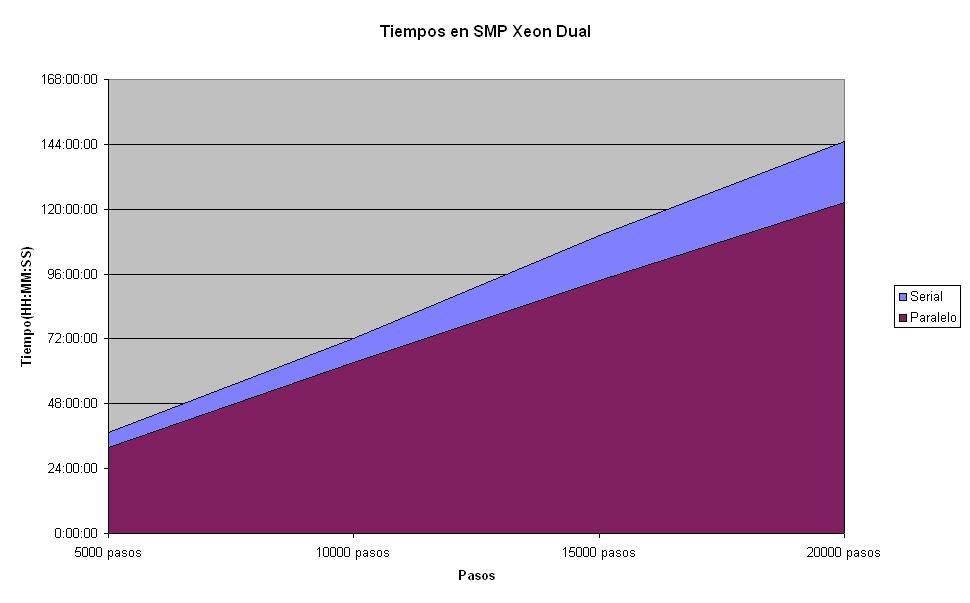
\includegraphics[keepaspectratio, width=14cm]{Papita}
\end{center}
\caption[Tiempos de ejecuci\'on en m\'aquina SMP Xeon Dual]{\small{Tiempos de ejecuci\'on total del programa con reordenamiento de c\'alculo en una m\'aquina SMP Xeon Dual con 7 \'atomos. Los resultados est\'an expresados en HH:MM:SS.}}
\label{fig:Papita}
\end{figure}

Como puede observarse, esta implementaci\'on es mucho m\'as r\'apida que de la de 128 bits debido a que no se utiliza emulaci\'on por software para realizar las operaciones. Tambi\'en puede observarse como la brecha de tiempos entre el programa serial y el paralelo tambi\'en se va abriendo conforme se agranda el dominio del problema. En las figuras \ref{fig:Speedup}, \ref{fig:Eficiencia}, \ref{fig:Overhead} y \ref{fig:OverheadP} se muestran diversas variables de performance asociadas a estas corridas.

\begin{figure}[ht!]
\begin{center}
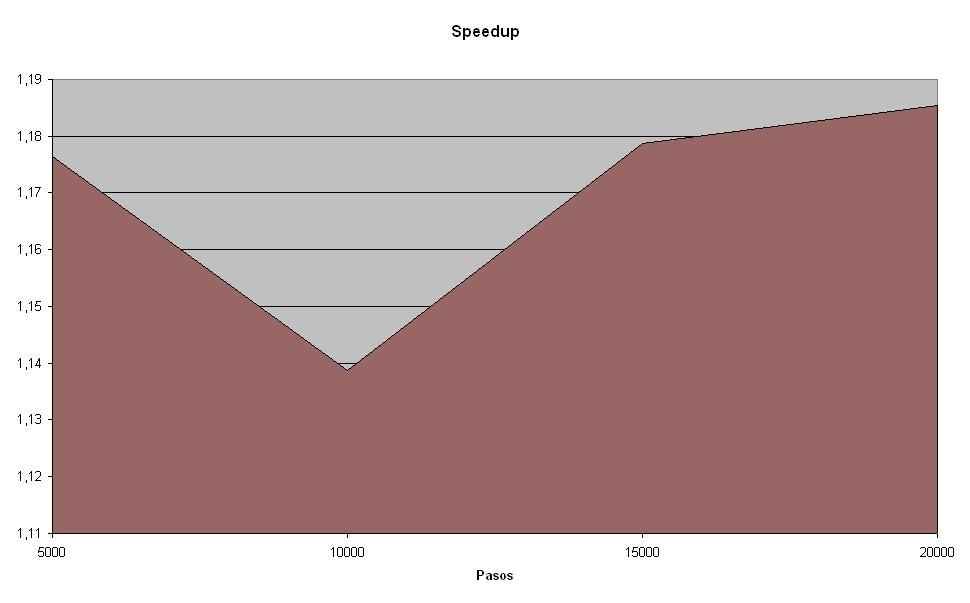
\includegraphics[keepaspectratio, width=14cm]{Speedup}
\end{center}
\caption[Speedup del programa con reordenamiento de c\'alculo en 2 procesos.]{\small{Speedup del programa con reordenamiento de c\'alculo en 2 procesos.}}
\label{fig:Speedup}
\end{figure}

\begin{figure}[ht!]
\begin{center}
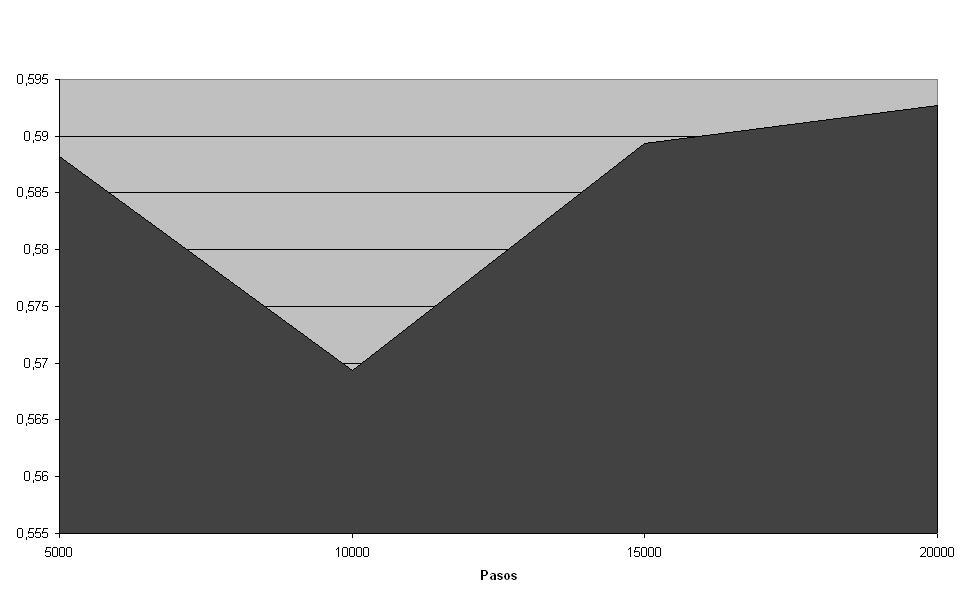
\includegraphics[keepaspectratio, width=14cm]{Eficiencia}
\end{center}
\caption[Eficiencia del programa con reordenamiento de c\'alculo en 2 procesos.]{\small{Eficiencia del programa con reordenamiento de c\'alculo en 2 procesos.}}
\label{fig:Eficiencia}
\end{figure}

\begin{figure}[ht!]
\begin{center}
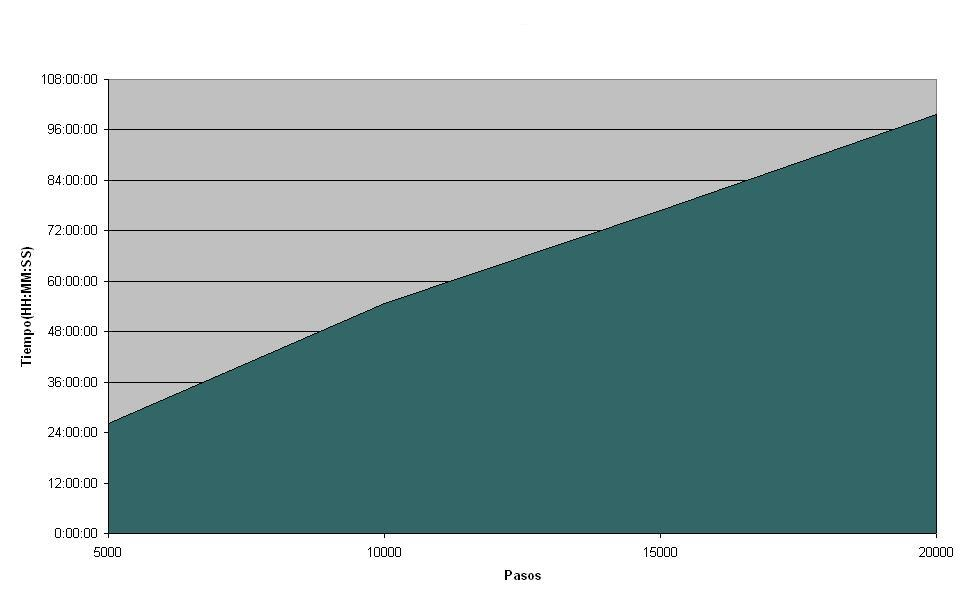
\includegraphics[keepaspectratio, width=14cm]{Overhead}
\end{center}
\caption[Overhead del programa con reordenamiento de c\'alculo en 2 procesos.]{\small{Overhead del programa con reordenamiento de c\'alculo en 2 procesos.}}
\label{fig:Overhead}
\end{figure}

\begin{figure}[ht!]
\begin{center}
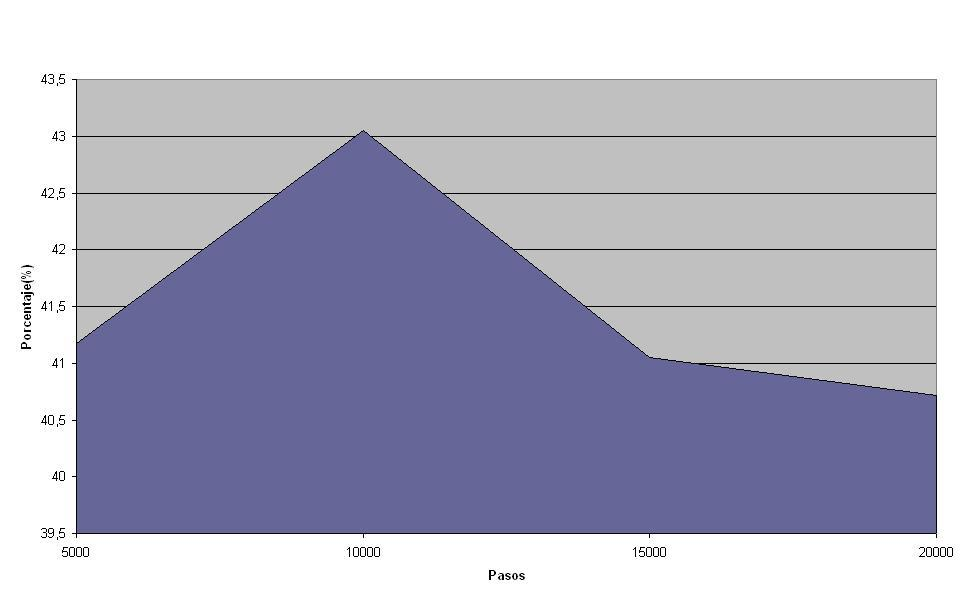
\includegraphics[keepaspectratio, width=14cm]{OverheadP}
\end{center}
\caption[Overhead del programa con reordenamiento de c\'alculo en 2 procesos.]{\small{Overhead del programa con reordenamiento de c\'alculo en 2 procesos.}}
\label{fig:OverheadP}
\end{figure}

Puede observarse en los gr\'aficos que cuando se realiz\'o la medici\'on con una ejecuci\'on de 10000 pasos el overhead en practicamente un 2\%. A pesar de que el gr\'afico porduce la sensaci\'on de que esta variaci\'on es muy grande no lo es realmente. Esta situaci\'on puede deberse al hecho de que la m\'aquina en la cual fueron realizadas las corridas tambi\'en es utilizada espor\'adicamente para realizar otros trabajos. Si bien se intent\'o que la m\'aquina no fuera utilizada por otras personas es posible que no haya sido este el caso y se haya corrido algun proceso corto que haya modificado los tiempos de ejecuci\'on del programa. A\'un as\'i, el speedup y la eficiencia medidas no son para nada despreciables y demuestran una ganancia en performance m\'as que interesante a los fines de la investigaci\'on futura de sistema de part\'iculas mayores. Por otro lado cabe aclarar que la utilizaci\'on por parte de otros usuarios de la SMP Xeon Dual no afecta el programa serial dado que el mismo es corrido en un solo procesador, mientras que los procesos de usuarios pueden correrse en el otro. En cambio, si afecta al programa paralelo dado que el mismo utiliza ambos procesadores, y si uno se retrasa debido al uso, el otro tambi\'en lo har\'a debido a la mensajer\'ia bloqueante y a la interacci\'on de ambos procesos.

Luego fueron realizadas mediciones en el cluster $Rocky$ del Laboratorio de Sistemas Complejos de la Facultad de Ciencias Exactas y Naturales de la UBA. El mismo est\'a compuesto por cuatro nodos AMD Opteron duales conectados por una red de Gigabit Ehernet.
Las corridas fueron realizadas con cuatro procesos en nodos distintos, es decir a raz\'on de un proceso en cada nodo, obteni\'endose los resultados que se pueden ver en la tabla \ref{tab:TiemposEjecucion3} y en la figura \ref{fig:RockyTiempos1}.

\begin{table}
\begin{center}
\begin{tabular}{|c|c|c|c|c|}
\hline
\ & \textbf{5000 pasos}& \textbf{10000 pasos}& \textbf{15000 pasos}& \textbf{20000 pasos}\\
\hline
\texttt{Serial} & 37:33 & 72:12 & 110:25 & 145:10 \\
\texttt{Paralelo}  & 31:55 & 63:24 & 93:40 & 122:27 \\
\hline
\end{tabular}
\end{center}
\caption[Tiempos de ejecuci\'on total del programa en 4 procesos]{\small{Tiempos de ejecuci\'on total del programa en 4 procesos.}}
\label{tab:TiemposEjecucion3}
\end{table}

\begin{figure}[ht!]
\begin{center}
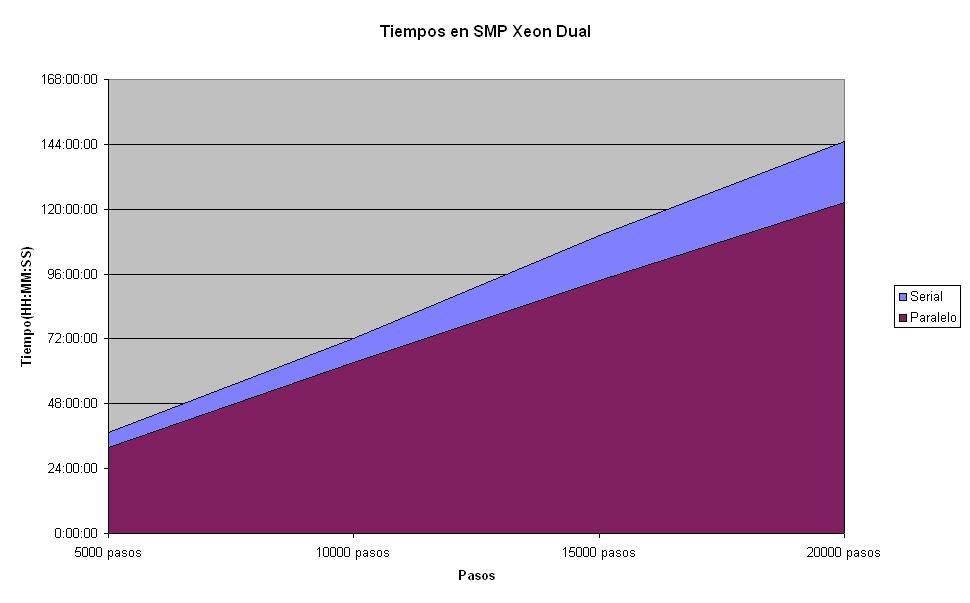
\includegraphics[keepaspectratio, width=14cm]{Papita}
\end{center}
\caption[Tiempos de ejecuci\'on total del programa en 4 procesos]{\small{Tiempos de ejecuci\'on total del programa en 4 procesos.}}
\label{fig:RockyTiempos1}
\end{figure}


A continuaci\'on fueron realizadas las mismas ejecuciones sobre el mismo cluster pero utilizando \'unicamente dos procesos en nodos distintos, obteni\'endose los siguientes resultados visibles en la tabla \ref{tab:TiemposEjecucion4} y en la figura \ref{fig:RockyTiempos2}.

\begin{table}
\begin{center}
\begin{tabular}{|c|c|c|c|c|}
\hline
\ & \textbf{5000 pasos}& \textbf{10000 pasos}& \textbf{15000 pasos}& \textbf{20000 pasos}\\
\hline
\texttt{Serial} & 37:33 & 72:12 & 110:25 & 145:10 \\
\texttt{Paralelo}  & 31:55 & 63:24 & 93:40 & 122:27 \\
\hline
\end{tabular}
\end{center}
\caption[Tiempos de ejecuci\'on total del programa en 2 procesos]{\small{Tiempos de ejecuci\'on total del programa en 2 procesos.}}
\label{tab:TiemposEjecucion4}
\end{table}

\begin{figure}[ht!]
\begin{center}
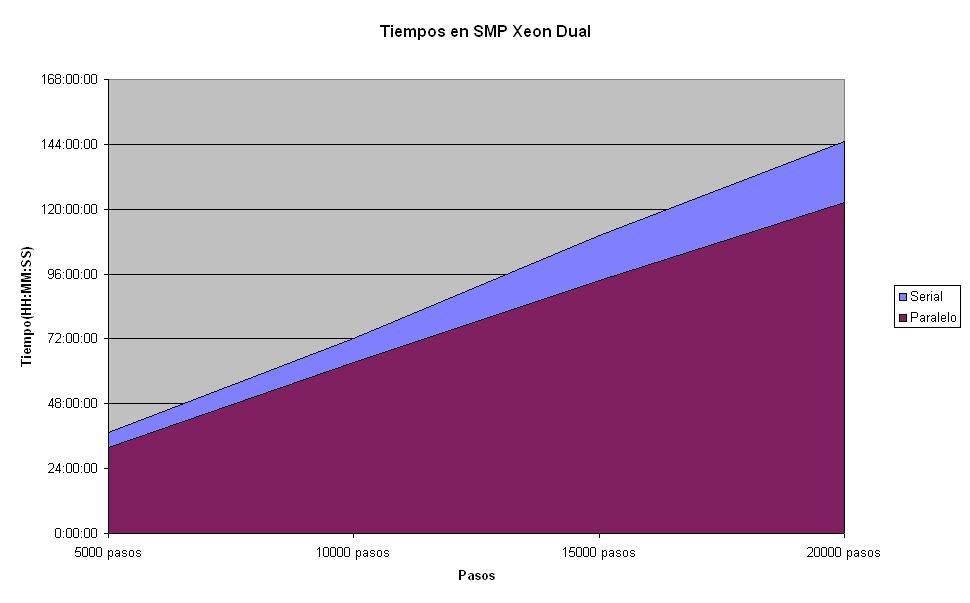
\includegraphics[keepaspectratio, width=14cm]{Papita}
\end{center}
\caption[Tiempos de ejecuci\'on total del programa en 2 procesos]{\small{Tiempos de ejecuci\'on total del programa en 2 procesos.}}
\label{fig:RockyTiempos2}
\end{figure}

Una vez obtenidos los datos de las ejecuciones del sistema en distintas configuraciones y entornos se pudieron obtener datos sobre \emph{speedup}, \emph{overhead} y \emph{eficiencia}, observables en las figuras \ref{fig:SpeedupRocky}, \ref{fig:EficienciaRocky}, \ref{fig:OverheadRocky} y \ref{fig:OverheadPRocky} respectivamente.

\begin{figure}[ht!]
\begin{center}
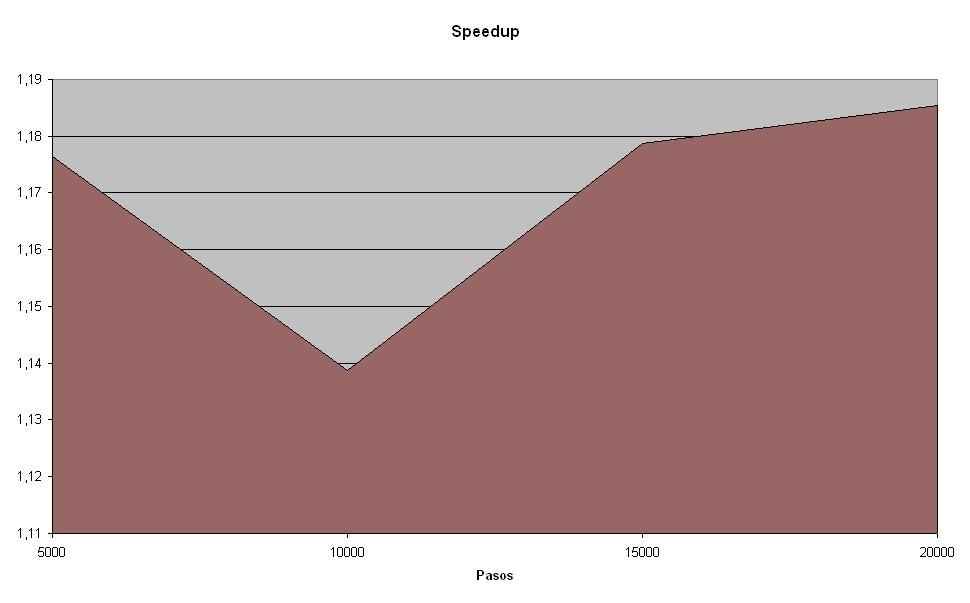
\includegraphics[keepaspectratio, width=14cm]{Speedup}
\end{center}
\caption[Speedup del programa con reordenamiento de c\'alculo en cluster de AMD Opteron Duales.]{\small{Speedup del programa con reordenamiento de c\'alculo en cluster de AMD Opteron Duales.}}
\label{fig:SpeedupRocky}
\end{figure}

\begin{figure}[ht!]
\begin{center}
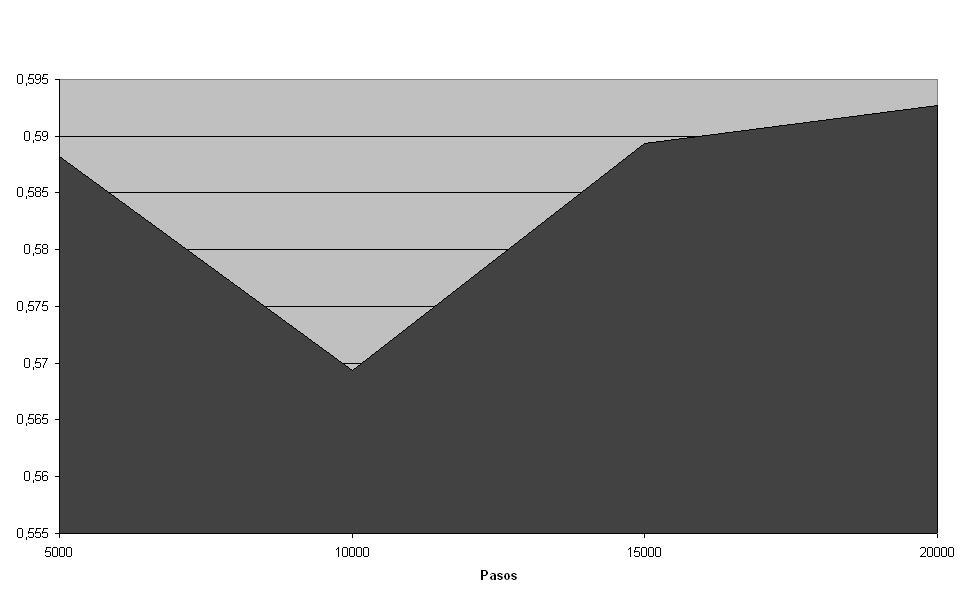
\includegraphics[keepaspectratio, width=14cm]{Eficiencia}
\end{center}
\caption[Eficiencia del programa con reordenamiento de c\'alculo en cluster de AMD Opteron Duales.]{\small{Eficiencia del programa con reordenamiento de c\'alculo en cluster de AMD Opteron Duales.}}
\label{fig:EficienciaRocky}
\end{figure}

\begin{figure}[ht!]
\begin{center}
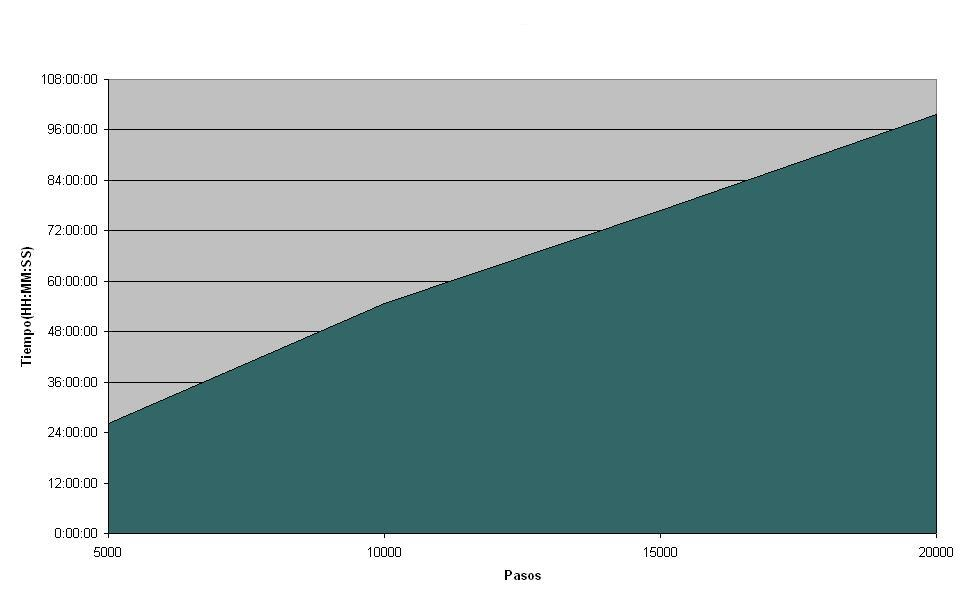
\includegraphics[keepaspectratio, width=14cm]{Overhead}
\end{center}
\caption[Overhead del programa con reordenamiento de c\'alculo en cluster de AMD Opteron Duales.]{\small{Overhead del programa con reordenamiento de c\'alculo en cluster de AMD Opteron Duales.}}
\label{fig:OverheadRocky}
\end{figure}

\begin{figure}[ht!]
\begin{center}
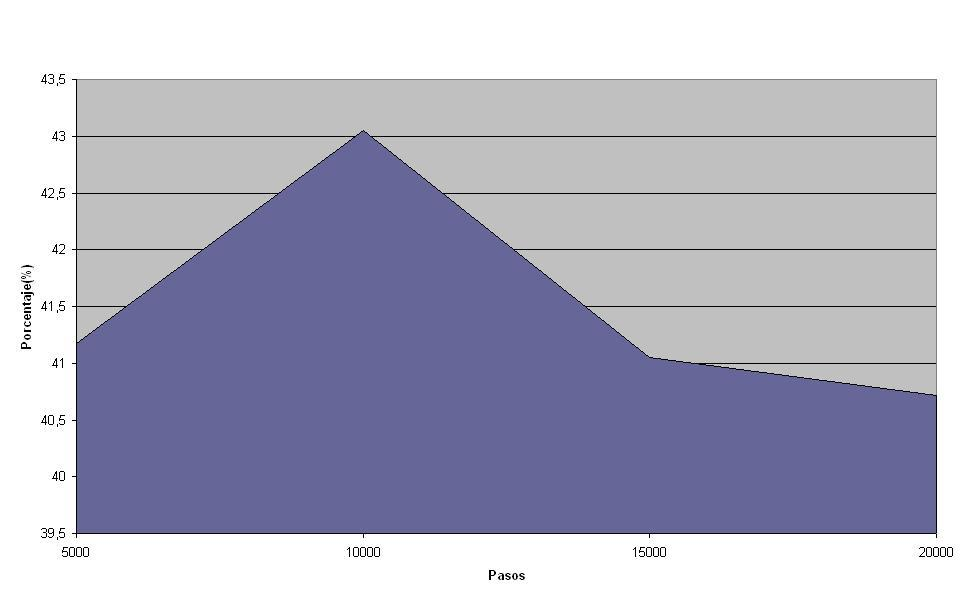
\includegraphics[keepaspectratio, width=14cm]{OverheadP}
\end{center}
\caption[Overhead del programa con reordenamiento de c\'alculo en cluster de AMD Opteron Duales.]{\small{Overhead del programa con reordenamiento de c\'alculo en cluster de AMD Opteron Duales.}}
\label{fig:OverheadPRocky}
\end{figure}


Puede observarse que conforme el dominio del problema crece la brecha entre los tiempos del sistema serial y los del paralelo se vuelven mayores. Quedar\'a a futuro la ejecuci\'on de un sistema de mayores dimensiones para completar el estudio sobre performance del sistema paralelizado para observar cual es l\'imite de procesamiento del nuevo programa con fines pr\'acticos. A simple vista puede observarse que para mayores dominios del problema los tiempos ahorrados por el sistema paralelo crecen significativamente con respecto al serial.

En contraparte a los resultados obtenidos puede observarse el gran overhead introducido en la versi\'on paralela del programa debido al pasaje de mensajes, lo cual hace que el $Speedup$ no sea lineal con respecto a la cantidad de procesos utilizados. Esto quiere decir que si el $Speedup$ fuera lineal, utilizando dos procesos el c\'alculo deber\'ia tardar la mitad de tiempo. \'Esta situaci\'on no se esta cumpliendo debido a que como muestran los gr\'aficos, el overhead var\'ia entre poco m\'as del 30\% y el 50\% del tiempo total, y a futuro queda una investigaci\'on m\'as profunda para intentar reducir el mismo. El overhead se produce no solo debido a la comunicaci\'on entre procesos sino tambi\'en al agregado de operaciones utilizadas para particionar el dominio del problema y posteriormente volver a unirlo. Sin embargo los costos de comunicaci\'on son mucho mayores a los de procesamiento, por lo cual generalmente se desprecian los \'ultimos. Sin embargo, en este caso en particular se ha podido observar que al tratar con grandes cantidades de datos, las operaciones agregadas produc\'ian un aumento significativo en el tiempo total de ejecuci\'on del programa paralelo y es por eso que se debi\'o analizar como reducir las mismas al m\'inimo posible. Por otra parte los costos de comunicaci\'on en un cluster como $Rocky$ son mayores a los presentes en una SMP Xeon Dual debido a que el primero posee buses externos de comunicaci\'on (lease por ejemplo cables) que son m\'as lentos que los buses internos utilizados en la segunda.

Finalmente, para demostrar la utilidad final del programa fueron realizadas corridas totalmente nuevas en diversos clusters y en la SMP Xeon Dual para contribuir con el procesamiento de datos a la investigaci\'on qu\'imica para la cual se hizo el programa serial. Estas corridas fueron desarrolladas por el grupo de qu\'imica inorg\'anica que provey\'o el programa serial y fueron supervisadas por los mismos mientras se realizaban para verificar la correctitud de los datos obtenidos.


Como trabajo a futuro se testear\'an dominios mayores y la ejecuci\'on de los mismos en un cluster de mayor magnitud, sin embargo esto no puede ser realizado de momento debido a falta de tiempo para realizar ejecuciones de gran envergadura.

Por otra parte podr\'ia investigarse a futuro la utilizaci\'on de mensajes no bloqueantes, ya que la metodolog\'ia actual (paso de mensajes bloqueantes) produce un overhead en el cual los procesos se encuentran inactivos. Sin embargo, la implementaci\'on de mensajes no bloqueantes requiere de un an\'alisis exhaustivo del problema para poder seleccionar zonas del programa en el que puedan solaparse c\'alculo y comunicaci\'on. Dado que la funci\'on que ha sido elegida como blanco de optimizaci\'on no requiere sincronizaci\'on intermedia, por el momento no hemos utilizado esta modalidad. Por otro lado la alta inestabilidad num\'erica del programa convierte este tipo de optimizaci\'on en un problema demasiado complejo para ser tratado en el presente trabajo. El motivo de esta aseveraci\'on es que al utilizar mensajes no bloqueantes el orden de operaciones se ve modificado, y como hemos explicado en secciones anteriores esto es causal de resultados no deseados e incorrectos.

\pagebreak
\chapter{Conclusiones}

De lo estudiado en el presente trabajo se desprenden diversas observaciones.

El programa serial es inestable num\'ericamente. Uno de los mayores problemas para realizar una soluci\'on paralela radic\'o en la inestabilidad num\'erica del programa original. Esto qued\'o demostrado al realizar diversos an\'alisis en los cuales se alteraban los \'ordenes de distintas operaciones y los resultados cambiaban radicalmente, al punto de obetener un resultado totalmente distinto, err\'oneo seg\'un los parametros esperados o directamente ninguno. A pesar de que entre los autores originales del sistema exist\'ia la noci\'on de existencia de estos problemas nunca se hab\'ia demostrado de forma contundente el mismo, lo cual fue un avance para la toma de conciencia y un planteo sobre la forma de trabajo y el rumbo futuro a seguir para eliminar los mismos.

Luego de investigar el tema con distintas personas y consultar con profesionales reconocidos en el \'area de m\'etodos num\'ericos se plantearon dos soluciones posibles y ambas fueron implementadas.

La primera versi\'on realizada alcanz\'o los objetivos de resultados, sin embargo al trabajar con n\'umeros de punto flotante de precis\'on cu\'adruple la performance del mismo se vi\'o agravada de forma notable. Esto se debi\'o a que no existen en la actualidad m\'aquinas que trabajen con esa precisi\'on en forma nativa sino que lo hacen por medio de emulaci\'on por software. Esta primera soluci\'on ser\'a utilizable a futuro si es que se inventan m\'aquinas con unidad de punto flotante que posean registros de 128 bits. En ese momento esta versi\'on ser\'a probablemente mejor en cuanto a performance y precisi\'on que la que finalmente fu\'e utilizada en este trabajo y se explicar\'a el porqu\'e. La versi\'on de 128 bits ya como se explic\'o tiene una mayor precisi\'on de variables, pero no solo eso, posee menos operaciones que la segunda soluci\'on implementada debido a que esta \'ultima utiliz\'o uh reordenamiento de c\'alculo que necesit\'o de una cierta cantidad de instrucciones con su consiguiente costo computacional.

Con la implementaci\'on que finalmente se utiliz\'o en este estudio se logr\'o una aproximaci\'on al sistema serial que aunque no otorga resultados exactamente iguales los mismos son muy similares. En esta implementaci\'on se opt\'o por ocasionar una p\'erdida de precisi\'on a cambio de la posibilidad de estudiar sistemas m\'as grandes. Esto es posible gracias a que la p\'erdida existente no es significativa, y los resultados obtenidos estan dentro de los par\'ametros aceptables.

Como pudo observarse, el algoritmo paralelo se vuelve m\'as efectivo conforme el dominio del problema crece. Esto se debe a que el overhead producido por la comunicaci\'on entre procesos se ve compensado por la cantidad de instrucciones ejecutadas en cada uno de los nodos.

El programa paralelo obtenido abre un abanico de posibilidades para poder resolver sistemas intratables hasta el momento, he aqu\'i su mejor caracter\'istica.
Adicionalmente, la performance del programa resulta razonable y el overhead producido se ve compensado por la ventaja de poder tratar sistemas cada vez m\'as grandes. 

Por otra parte pudo observarse que el pico de eficiencia del programa paralelo se obtuvo en una m\'aquina sin buses externos, debido a que los costos de comunicaci\'on afectan la performance. Es por este motivo que para diversas corridas nuevas se utiliz\'o una SMP Xeon Dual debido a que la ganancia de la misma era de un 15\% aproximadamente lo cual reduc\'ia los tiempos de investigaci\'on de forma notoria. Sin embargo esto no quiere decir que a futuro no se logre una mejor performance cuando la comunicaci\'on entre nodos de un cluster mejore y convenga m\'as la utilizaci\'on de varios nodos en vez de solo utilizar una m\'aquina dual.

\pagebreak
\chapter{Trabajo futuro}

Como se puede observar en el profiling existen diversas rutinas que pueden intentarse paralelizar. Uno de los ejemplos puntuales son las rutinas $IntSol$ e $IntSolg$ que consumen alrededor del 15\% del tiempo total. Otras rutinas son las del tipo de la $int3$ que invocan en gran n\'umero a la funci\'on $funct$ lo cual produce un consumo del 5\% del tiempo total. Por otra parte queda como trabajo de desarrollo a futuro el uso de determinadas variables en memoria en vez de el c\'alculo de las mismas cada vez que son solicitadas, lo cual esta produciendo una perdida de performance importante.
Finalmente como se mencion\'o con anterioridad queda pendiente el estudio de la utilizaci\'on de mensajer\'ia no bloqueante asi tambi\'en como la prueba del sistema en otras tecnolog\'ias para observar las diversas variables de performance(speedup, overhead, eficiencia).

\pagebreak
\appendix

\chapter{Glosario\label{Glosario}}
\begin{itemize}

\item Cluster: Un cluster es un grupo de equipos individuales que trabajan en cooperaci\'on para proporcionar una mayor capacidad inform\'atica y garantizar la disponibilidad cont\'inua de las aplicaciones o los servicios escenciales. La principal ventaja de un cluster radica en el multiprocesamiento masivamente paralelo (muchos procesadores, memoria distribuida y red). Ver Cap\'itulo \ref{Simulacion}

\item Beowulf: Cluster Beowulf no es un software especial, ni una topolog\'ia de red, ni un n\'ucleo modificado. Beowulf es una tecnolog\'ia dise\~nada para agrupar computadores basados bajo el sistema operativo Linux para formar un supercomputador virtual paralelo. Beowulf posee una arquitectura basada en multicomputadores el cual puede ser utilizado para la computaci\'on paralela. Este sistema consiste de un nodo maestro y uno o m\'as nodos esclavos conectados a trav\'es de una red Ethernet u otra topolog\'ia de red. Esta construido con componentes de hardware comunes, como ser cualquier PC capaz de ejecutar Linux, adaptadores de Ethernet y switches est\'andares. Una de las diferencias principales entre Beowulf y un cluster de estaciones de trabajo (COW, Cluster Of Workstations) es el hecho de que Beowulf se comporta m\'as como una sola m\'aquina que como muchas estaciones de trabajo conectadas. En la mayor\'ia de los casos los nodos esclavos no tienen monitores o teclados y son accedidos solamente v\'ia remota o por terminal serie. El nodo maestro controla el cluster entero y presta servicios de sistemas de archivos a los nodos esclavos. Ver Cap\'itulo \ref{Simulacion}

\item M\'etodos h\'ibridos: Uno de los principales objetivos de la Qu\'imica Computacional es el de obtener medidas sobre propiedades f�sco-qu\'imicas (tanto macrosc\'opicas como microsc\'opicas) mediante la aplicaci\'on de modelos te\'oricos al estudio de sistemas at\'omicos o moleculares. Podemos agrupar estos modelos te\'oricos como pertenecientes a dos grandes grupos, en funci\'on de la teor�a f\'isica de la que hacen uso:

\begin{enumerate}
\item M\'etodos basados en la Mec\'anica Cu\'antica
\item M\'etodos basados en la Mec\'anica Cl\'asica
\end{enumerate}

Los primeros, como indica su nombre, se han desarrollado a partir de la formulaci\'on de la mec\'anica cu\'antica aplicada. M\'etodos h\'ibridos QM/MM proviene del ingl\'es Quantum Mechanics / Molecular Mechanics. Esta metodolog\'ia consiste en combinar c\'alculos de estructura electr\'onica con la mec\'anica molecular cl\'asica a trav\'es de un Hamiltoniano h\'ibrido ($H_{qm-mm}$).Ver Cap\'itulo \ref{Metodologia}

\item Onda plana: Se denomina as\'i a las ondas que poseen una dimensi\'on, o, lo que es lo mismo, que su direcci\'on de propagaci\'on es \'unica. Ver Cap\'itulo \ref{Introduccion}.

\item M\'etodo de Hartree-Fock: Es un procedimiento iterativo para calcular la mejor soluci\'on a la ecuaci\'on de Schr�dinger independiente del tiempo, para mol\'eculas aisladas, tanto en su estado fundamental como en estado de excitaci\'on. Este m\'etodo permite calcular la energ\'ia de intercambio de la mol\'ecula de forma exacta, pero no tiene en cuenta el efecto de la correlaci\'on electr\'onica. HF realiza una aproximaci\'on de la energ\'ia total de la mol\'ecula calculando la interacci�n de un \'unico electr\'on con el resto de los electrones del sistema mediante el promedio de una interacci\'on entre dos cuerpos. Ver Cap\'itulo \ref{Introduccion}.

\item Ecuaci\'on de Schr�dinger: desarrollada por el f\'isico austr\'iaco Erwin Rudolf Josef Alexander Schr�dinger en 1925, describe la dependencia temporal de los sistemas mecanocu\'anticos. Es de importancia central en la teor\'ia de la mec\'anica cu\'antica, donde representa un papel an\'alogo a las leyes de Newton en la mec\'anica cl\'asica.

\item Hamiltoniano: En mec\'anica cu\'antica es el operador que retorna total de energ\'ia de un sistema en forma de un Eigen-valor. Ver Cap\'itulo \ref{Metodologia}.

\end{itemize}


\pagebreak
\chapter{Hardware y Software utilizados}

\section{Hardware}
Papita: Intel SMP Xeon Dual, cedida gentilmente por Intel Argentina.

FIU-PG (Florida): 17 Intel SMP Xeon Dual HT 2.6GHz, 1.96Gb RAM

\section{Software}

Lenguaje de programaci\'on: Fortran77, Fortran90

Compilador: g77 3.4.4, Intel Fortran Compiler

Sistema Operativo: Gentoo Linux 3.4.4

Implementaciones utilizadas de MPI: LAM-MPI 7.0.4 y MPICH 1.2.7p1


\pagebreak

\printindex

\pagebreak
\listoffigures

\listoftables


\pagebreak

\bibliographystyle{unsrt}
\bibliography{bibliografia}

\nocite{Newman}
\nocite{Probstein}
\nocite{Szabo99}
\nocite{Perdew96}
\nocite{Lee88}
\nocite{Baez94}
\nocite{Jarzinski1997}
\nocite{Liphardt2002}
\nocite{Koppenol93}
\nocite{Squadrito95}
\nocite{Keith69}
\nocite{Lymar98}
\nocite{Bonini99}
\nocite{Greengard88}
\nocite{Lambert76}
\nocite{Wiki}

\end{document}